\documentclass[hyperref={pdfpagelabels=false}]{beamer}
\usepackage{CJKutf8}
\usepackage[english]{babel}
\usepackage{xcolor}
\usepackage{lmodern}
\usepackage{amssymb}
\usepackage[makeroom]{cancel} %for crossing symbols
\usepackage{leftindex} %For leftindex, making it possible to have nicely aligned left subscripts
%\usepackage{calligra}
%\DeclareMathAlphabet{\mathcalligra}{T1}{calligra}{m}{n} %For small \mathcal letters
\makeatletter
\DeclareFontEncoding{LS1}{}{}
\DeclareFontSubstitution{LS1}{stix}{m}{n}
\DeclareMathAlphabet{\mathKel}{LS1}{stixscr}{m}{n}
\DeclareMathAlphabet{\mathcal}{LS1}{stixscr}{m}{n}
\usepackage{amsthm}
\usepackage{amsmath}
%\usepackage{mathabx}
\usepackage{stmaryrd}
\usepackage{amsbsy}
\usepackage{dsfont}
\usepackage{mathtools} %für mathclap und coloneqq
%\usepackage{amsbsy}
\usepackage{mleftright} %Distanz zu \left \right weg
\usepackage{tikz-cd}

\usepackage{tabularx} %Automatic line break of tables using X instead c l r
%\usepackage{longtable} %table auf mehreren Seiten
%\usepackage{ltxtable} %Combination of both above
\usepackage{xcolor, colortbl}

%Für die ganzen Diagramme
\usepackage{pgfplots}
\usepackage{graphicx} %Für raisebox, vertical displacement of figures
\usetikzlibrary{decorations.markings, decorations.text,calc,arrows.meta}

\definecolor{Gray}{gray}{0.85}
%\usepackage[style=authortitle-icomp]{biblatex}
%\usepackage[babel,german=guillemets]{csquotes}

\setcounter{tocdepth}{1}
%\setcounter{tocdepth}{5}
%\setcounter{secnumdepth}{4}
%\setcounter{secnumdepth}{5}
\usepackage[backend=biber, style=numeric]{biblatex}
\addbibresource{Literatur.bib}
\newcommand{\footlineextra}[1]{
    \begin{tikzpicture}[remember picture,overlay]
        \node[yshift=2ex,anchor=south west] at (current page.south west) {\usebeamerfont{author in head/foot}\hspace{2ex}#1};
    \end{tikzpicture}
}

\newcommand\insertreferences{}
\setbeamertemplate{footline}{%
  \leavevmode%
  \hbox{%
  \begin{beamercolorbox}[wd=.09\paperwidth, ht=5ex,dp=1ex,center, sep=1.4ex]{author in head/foot}%
    \usebeamerfont{author in head/foot}
		%\vfill
		%Sources
		%\vfill
		Sources
  \end{beamercolorbox}%
  \begin{beamercolorbox}[wd=.91\paperwidth,ht=5ex,dp=1ex,center]{title in head/foot}%
    \usebeamerfont{title in head/foot}
    \insertreferences

  \end{beamercolorbox}
}
}


%%% Transition slides
\AtBeginSection[]{
  \begin{frame}
  %\vfill
	\thispagestyle{empty}
  \centering
  \begin{beamercolorbox}[sep=8pt,center,shadow=true,rounded=true]{title}
    \usebeamerfont{title}\insertsection\par%
  \end{beamercolorbox}
  %\vfill
  \end{frame}
}

\title{Curved Yang-Mills gauge theories and their recent applications}   
\subtitle{}   
\author{Simon-Raphael Fischer} 
\institute{
\begin{figure}
	\centering
		
\includegraphics[width=.50\textwidth]{NCTS.png}
	\label{fig:NCTS}
\end{figure}
\begin{CJK*}{UTF8}{bkai}國家理論科學研究中心\end{CJK*}\\
National Center for Theoretical Sciences (National Taiwan University)
}
\date{} 
%\date{Le lundi 31 mai 2021} 

% zusaetzlich ist das usepackage{beamerthemeshadow} eingebunden 
%\usepackage{beamerthemeIlmenau}
%\usepackage{beamerthemeshadow}
\usepackage{beamerthemeDarmstadt}

%  \beamersetuncovermixins{\opaqueness<1>{25}}{\opaqueness<2->{15}}
%  sorgt dafuer das die Elemente die erst noch (zukuenftig) kommen 
%  nur schwach angedeutet erscheinen 
\beamersetuncovermixins{\opaqueness<1>{25}}{\opaqueness<2->{15}}
% klappt auch bei Tabellen, wenn teTeX verwendent wird\ldots

\beamertemplatenavigationsymbolsempty %Damit sind die kleinen Navigationssymbole unten weg

%\usesectionheadtemplate{}{}
%\usesubsectionheadtemplate{}{}

\def\be{\begin{equation}}
\def\ee{\end{equation}}
\def\bs{\begin{subequations}}
\def\es{\end{subequations}}
\def\ba#1\ea{\begin{align}#1\end{align}}
\def\bes{\begin{equation*}}
\def\ees{\end{equation*}}
\def\bas#1\eas{\begin{align*}#1\end{align*}}

\AtBeginEnvironment{remark}{%
  \setbeamercolor{block title}{use=example text,fg=black,bg=yellow!75!black}
  \setbeamercolor{block body}{parent=normal text,use=block title example,bg=yellow!10}
}

\renewcommand{\qedsymbol}{}
\theoremstyle{plain}
\newtheorem{conjecture}[theorem]{Conjecture}
\newtheorem{proposition}[theorem]{Proposition}
%\newtheorem{definition}[theorem]{Definition}
\theoremstyle{remark}
\newtheorem*{remark}{Remarks}
\newtheorem*{idea}{Idea}
\newtheorem*{motivation}{Motivation}
\newtheorem*{summary}{Summary}
\newtheorem*{situation}{Situation}
\newtheorem*{lab}{Situation: Lie algebra bundles}
\newtheorem*{question}{Question}
\newtheorem*{fieldredefinition}{Field Redefinition}
\newtheorem*{construction}{Construction}
\newtheorem*{aim}{Aim}
\newtheorem*{BackToTheRoots}{Back to the roots}

\AtBeginEnvironment{BackToTheRoots}{%
  \setbeamercolor{block title}{use=example text,fg=black,bg=pink!75!black}
  \setbeamercolor{block body}{parent=normal text,use=block title example,bg=pink!10}
}
\AtBeginEnvironment{idea}{%
  \setbeamercolor{block title}{use=example text,fg=black,bg=pink!75!black}
  \setbeamercolor{block body}{parent=normal text,use=block title example,bg=pink!10}
}

%\theoremstyle{definition}
%\newtheorem{definition}[theorem]{Definition}
%\newtheorem*{SecondIn}{Second Inequality}

%mathrm mit mathup ersetzen, damit die font passt
\renewcommand\familydefault{\sfdefault} %comment to see the difference
\DeclareMathAlphabet      {\mathup}{OT1}{\familydefault}{m}{n}


\begin{document}


\begin{frame}
\thispagestyle{empty}
\titlepage
\end{frame} 


{
\setbeamertemplate{footline}{}
\begin{frame}
\frametitle{Table of contents}
\tableofcontents
\end{frame} 
}

\section[Infinitesimal cYM]{Infinitesimal Version}

{
\setbeamertemplate{footline}{}
\begin{frame}{\textbf{Infinitesimal} curved Yang-Mills-Higgs gauge theory}
\centering
\begin{tikzpicture}
\filldraw [fill=gray!10!white, draw=black] plot [smooth cycle] coordinates {(5,0.25) (6,0.35) (6.5, 0.2) (7,0.5) (7,1.65) (6.5,2.75) (5.8,2.75) (5.3,1.45) (4.8,0.85) } node at (6.2,1.7) {$(N, g)$} node at (6.2, 3.2) {Riemannian manifold};
\path[->] (2.6,1.7) edge [bend left] node[above] {Higgs field} node[below] {$\Psi$} (5.0,1.7);

\filldraw [fill=gray!10!white, draw=black] (-0.2,.5) to[bend left] (1.3,2.85) to[bend left] (2.7,2) to[bend right] (1.8,.5) to[bend right] cycle node at (1.2,1.7) {$(M, \eta)$} node at (1.2, 3.2) {Spacetime};
\path[->] (0.7,0.5) edge [bend right] node[left] {$A \in \Omega^1$} node[right] {Gauge bosons} (0.7, -1.5);
\filldraw [fill=gray, draw=black] (5.2, .7) circle (0.2);
\path[->] (2.5,-1.5) edge [bend right] node[right] {action $\gamma$} (5.2, .7);
\draw (-0.2,-1.7)-- (1.25, -1.7) node[below] {Lie algebra $\mathfrak{g}$} --(2.7,-1.7);

\tikzset{shift={(5,-3)}} %Change position of the next drawing
\begin{axis}[ scale = 0.6,
            hide axis,
            %axis lines=middle,
%            axis on top,
%            axis line style={blue,dashed,thick},
%            ymin=-2,ymax=2,
%            xmin=-2,xmax=2,
%            zmin=-2,zmax=2,
            samples=40,
            domain=0:360,
            y domain=0:1.25,clip=false
        ]
        \addplot3 [surf, shader=flat, draw=black, fill=gray!10!white, z buffer=sort]
           ({sin(x)*y}, {cos(x)*y}, {(y^2-1)^2});
        \draw[blue,thick,dashed] (axis cs:0,0,0) -- (axis cs:1,0,0)
                    node[below,font=\footnotesize]{};
        \draw[blue,thick,-stealth] (axis cs:1,0,0) -- (axis cs:1.3,0,0)
                    node[above,font=\footnotesize]{};
        \draw[blue,thick,dashed] (axis cs:0,0,0) -- (axis cs:0,-1,0)
                    node[left=2mm,font=\footnotesize]{}; %{Label} am Ende 
        \draw[blue,thick,-stealth] (axis cs:0,-1,0) -- (axis cs:0,-1.5,0)
                    node[right=1mm,font=\footnotesize]{};
        \draw[blue,thick,dashed] (axis cs:0,0,0) -- (axis cs:0,0,1)
                    %node[left=2mm,font=\footnotesize]{$\phi_{\text{RE}}$}
                    ;
        \draw[blue,thick,-stealth] (axis cs:0,0,1) -- (axis cs:0,0,1.3)
                    node[right,font=\footnotesize]{$\mathcal{V}$};
        \end{axis}
\end{tikzpicture}

\end{frame}

\begin{frame}{Guide: Infinitesimal curved Yang-Mills-Higgs gauge theory}
\setbeamercovered{invisible}
\begin{table}[h!]
		\begin{tabularx}{\textwidth}{X X}
			\rowcolor{gray}
			Classical formalism & CYMH GT \\
			Lie algebra $\mathfrak{g}$ as $M \times \mathfrak{g}$ & Lie algebroid $E \to N$ \\
			\rowcolor{Gray}
			$\mathfrak{g}$-action $\gamma$ & Anchor $\rho$ of $E$ \\ 
			\rowcolor{Gray}
			& \& $E$-connections \\
			Canonical flat connection $\nabla^0$ on $M \times \mathfrak{g}$ & General connection $\nabla$ on $E$
		\end{tabularx}
\end{table}
\pause
\begin{remark}[Why a "curved theory"?]
Usually, the field strength $F$ is given by (abelian, for simplicity)
\bas
F
&\coloneqq
\mathrm{d}A
=
\mathrm{d}^{\nabla^0}A.
\eas
$\rightsquigarrow$ We will use a general connection $\nabla$ instead of $\nabla^0$, and $\nabla$ may not be flat.
\end{remark}
\end{frame}
}

\subsection{Mathematical basics}

\renewcommand\insertreferences{{\tiny Ana Cannas Da Silva, Alan Weinstein. \textit{Geometric models for noncommutative algebras}, \newline volume 10. American Mathematical Society, 1999.}}

\begin{frame}
%Instead of Lie algebras we want to use:
\begin{definition}[Lie algebroids]
Let $E \to N$ be a vector bundle. Then $E$ is a Lie algebroid, if there is a bundle map $\rho: E \to \mathrm{T}N$, called the \textbf{anchor}, and a Lie algebra structure on $\Gamma(E)$ with Lie bracket $\mleft[\cdot, \cdot\mright]_E$ satisfying
\ba
  \mleft[\mu, f \nu\mright]_E = f \mleft[\mu, \nu\mright]_E + \mathcal{L}_{\rho(\mu)}(f) ~ \nu
\label{eq:E-Leibniz}
\ea
for all $f \in C^\infty(N)$ and $\mu, \nu \in \Gamma(E)$.
\end{definition}
\pause
\begin{example}
\begin{itemize}[<+->]
	\item $E = \mathrm{T}N$, $\rho = \mathds{1}_{\mathrm{T}N}$
	\item $E$ a bundle of Lie algebras, $\rho = 0$
\end{itemize}
\end{example}
\end{frame}
%
%\renewcommand\insertreferences{{\tiny Yvette Kosmann-Schwarzbach and Franco Magri. Poisson-Nijenhuis structures. \newline \textit{In Annales de l’IHP Physique théorique}, volume 53, pages 35–81, 1990.}}
%
%\begin{frame}
%As for an action $\gamma: \mathfrak{g} \to \mathfrak{X}(N)$ we have:
%\begin{proposition}[Anchor as homomorphism]
%$\rho: \Gamma(E) \to \mathfrak{X}(N)$ is a homomorphism of Lie algebras.
%\end{proposition}
%\end{frame}

\renewcommand\insertreferences{{\tiny Ana Cannas Da Silva, Alan Weinstein. \textit{Geometric models for noncommutative algebras}, \newline volume 10. American Mathematical Society, 1999.}}

\begin{frame}
The classical formalism will correspond to:
\begin{proposition}[Action Lie algebroids]
Let $\mleft(\mathfrak{g}, \mleft[\cdot, \cdot \mright]_{\mathfrak{g}}\mright)$ be a Lie algebra with a $\mathfrak{g}$-action $\gamma$ on $N$. Then there is a \textbf{unique} Lie algebroid structure on $E \coloneqq N \times \mathfrak{g}$ as a vector bundle over $N$ such that
\ba
\rho(\nu)
&=
\gamma(\nu),
\\
\mleft[\mu, \nu\mright]_E
&=
\mleft[\mu, \nu\mright]_{\mathfrak{g}}
\ea
for all constant sections $\mu, \nu \in \Gamma(E)$.
\end{proposition}
\end{frame}

{
\setbeamertemplate{footline}{}
\begin{frame}
\begin{table}[h!]
		\begin{tabularx}{\textwidth}{X X}
			\rowcolor{gray}
			Classical formalism & CYMH GT \\
			Lie algebra $\mathfrak{g}$ as $M \times \mathfrak{g}$ & Lie algebroid $E \to N$ \\
			\rowcolor{Gray}
			$\mathfrak{g}$-action $\gamma$ & Anchor $\rho$ of $E$ \\ 
			\rowcolor{Gray}
			& \& \textbf{$E$-connections} as lift of $\rho$ \\
			Canonical flat connection $\nabla^0$ on $M \times \mathfrak{g}$ & General connection $\nabla$ on $E$
		\end{tabularx}
\end{table}
			%\newline
			\pause
		$\rightsquigarrow$ $E$-connections similar to vector bundle connections but Leibniz rule along $\rho$, \textit{i.e.}~only lifting vector fields in the image of $\rho$
\end{frame}
}

\renewcommand\insertreferences{{ Mohamed Boucetta. Riemannian geometry of Lie algebroids. \newline \textit{Journal of the Egyptian Mathematical Society}, 19(1-2):57–70, 2011. }}

\begin{frame}
\begin{example}[$E$-connection ${}^E\nabla$ on $V$]
$\nabla^\prime$ a vector bundle connection on $V \to N$, then
\ba
{}^E\nabla_\nu v
&\coloneqq
\nabla^\prime_{\rho(\nu)} v
\ea
for all $\nu \in \Gamma(E)$ and $v \in \Gamma(V)$. In short denoted by $\nabla^\prime_\rho$.
\end{example}
\end{frame}

\renewcommand\insertreferences{{\tiny Camilo Arias Abad, Marius Crainic. Representations up to homotopy of Lie algebroids. \newline \textit{Journal für die reine und angewandte Mathematik (Crelles Journal)}, 2012(663):91–126, 2012.}}

\begin{frame}
\begin{example}
For $\nabla$ a connection on $E$ we have the \textbf{basic connection} given as a pair of $E$-connections on $E$ and on $\mathrm{T}N$ by
\ba
\nabla^{\mathrm{bas}}_\nu \mu
&\coloneqq
\mleft[ \nu, \mu \mright]_E
	+ \nabla_{\rho(\mu)} \nu,
\\
\nabla^{\mathrm{bas}}_\nu X
&\coloneqq
\mleft[ \rho(\nu), X \mright]
	+ \rho\mleft(\nabla_{X} \nu\mright)
\ea
for all $X \in \mathfrak{X}(N)$ and $\nu, \mu \in \Gamma(E)$.
\end{example}
\pause
\begin{remark}[Encoding of Lie algebra representations]
Test this with trivial bundles and canonical flat connection $\nabla^0$, \textit{i.e.}~$E = N \times \mathfrak{g}$ and $\nabla^0 \nu = 0$ for constant sections $\nu$.
\end{remark}
\end{frame}

%\renewcommand\insertreferences{{\tiny Camilo Arias Abad, Marius Crainic. Representations up to homotopy of Lie algebroids. \newline \textit{Journal für die reine und angewandte Mathematik (Crelles Journal)}, 2012(663):91–126, 2012.}}
\begin{frame}
\begin{definition}[Basic curvature]
Let $\nabla$ be a connection on $E$.
The \textbf{basic curvature $R_\nabla^{\mathrm{bas}}$} is defined as an element of $\Gamma\left(\bigwedge^2E^* \otimes \mathrm{T}^*N \otimes E \right)$ by
\ba
R^{\mathrm{bas}}_\nabla(\mu, \nu) X
&\coloneqq
\nabla_X\mleft(\mleft[\mu, \nu\mright]_E\mright) 
	- \mleft[ \nabla_X \mu, \nu \mright]_E 
	- \mleft[ \mu, \nabla_X \nu \mright]_E 
\nonumber\\
&\hspace{1cm}
	- \nabla_{\nabla^{\mathrm{bas}}_\nu X} \mu 
	+ \nabla_{\nabla^{\mathrm{bas}}_\mu X} \nu,
\ea
where $\mu, \nu \in \Gamma(E)$ and $X \in \mathfrak{X}(N)$.
\end{definition}

\pause
\begin{proposition}
We recover the curvature of the basic connection:
\ba
R_{\nabla^{\mathrm{bas}}}
&=
\mleft\{
\begin{array}{ll}
- R_\nabla^{\mathrm{bas}}(\cdot, \cdot) \circ \rho, & \text{on $E$}, \\
- \rho \circ R_\nabla^{\mathrm{bas}}, & \text{on $\mathrm{T}N$}.
\end{array}
\mright.
\ea
\end{proposition}
\end{frame}

\subsection{Curved Yang-Mills-Higgs gauge theory}

{
\makeatletter
\setbeamertemplate{footline}
{
  \leavevmode%
  \hbox{%
  \begin{beamercolorbox}[wd=.09\paperwidth,ht=2.25ex,dp=1ex,center]{author in head/foot}%
    \usebeamerfont{author in head/foot}
		Sources
  \end{beamercolorbox}%
  \begin{beamercolorbox}[wd=.91\paperwidth,ht=2.25ex,dp=1ex,center]{title in head/foot}%
    \usebeamerfont{title in head/foot}
		Alexei Kotov and Thomas Strobl. Curving Yang-Mills-Higgs gauge theories. \textit{Physical Review D}, 92(8):085032, 2015.
  \end{beamercolorbox}%
  %\begin{beamercolorbox}[wd=.175\paperwidth,ht=2.25ex,dp=1ex,right]{date in head/foot}%
    %\usebeamerfont{date in head/foot}\insertshortdate{}\hspace*{2em}
    %%\insertframenumber{} 
		%%/ \inserttotalframenumber\hspace*{2ex} 
  %\end{beamercolorbox}
	}%
  \vskip0pt%
}
\begin{frame}
\begin{definition}[Space of fields]
Fields are a pair consisting of:
\begin{itemize}[<+->]
	\item Higgs field $\Phi \in C^\infty(M;N)$
	\item Field of gauge bosons $A \in \Omega^1(M; \Phi^*E)$
\end{itemize}
\end{definition}
%\end{frame}
\pause
%\begin{frame}
\begin{definition}[Minimal coupling]
\textbf{Minimal coupling} $\mathfrak{D}$, $(\Phi, A) \mapsto \mathfrak{D}(\Phi, A) \in \Omega^1(M; \Phi^*\mathrm{T}N)$, by
\ba
\mathfrak{D}(\Phi, A)
&\coloneqq
\mathfrak{D}^A \Phi
\coloneqq
\mathrm{D}\Phi
	- (\Phi^*\rho)(A),
\ea
where $\mathrm{D}\Phi: \mathrm{T}M \to \mathrm{T}N$ is the tangent map.
\end{definition}
\end{frame}

\begin{frame}
\setbeamercovered{invisible}
\begin{definition}[Field strength]
Let $\nabla$ be a connection on $E$. We define the \textbf{field strength $F$}, $(\Phi, A) \mapsto F(\Phi, A) \in \Omega^2(M; \Phi^*E)$, by
\ba
F(\Phi, A)
\coloneqq
\mathrm{d}^{\Phi^*\nabla} A
	+ \frac{1}{2} \mleft( \Phi^* t_{\nabla^{\mathrm{bas}}} \mright)\mleft( A \stackrel{\wedge}{,} A \mright),
\ea
where $t_{\nabla^{\mathrm{bas}}}$ is the torsion of $\nabla^{\mathrm{bas}}$ on $E$ and $\mathrm{d}^{\Phi^*\nabla}$ the exterior covariant derivative of $\Phi^*\nabla$.
\end{definition}
\pause
\begin{definition}[Generalised field strength]
Let $\zeta$ be an element of $\Omega^2(N; E)$, then we define the \textbf{generalised field strength $\mathcal{F}$} by
\ba
\mathcal{F}(\Phi,A)
&\coloneqq
F(\Phi, A)
	+ \frac{1}{2} (\Phi^*\zeta)\mleft( \mathfrak{D}^A \Phi \stackrel{\wedge}{,} \mathfrak{D}^A \Phi \mright).
\ea
\end{definition}
\end{frame}

\begin{frame}
\begin{definition}[Curved Yang-Mills-Higgs (CYMH) Lagrangian]
Let $\kappa$ be a fibre metric on $E$, then the \textbf{curved Yang-Mills-Higgs Lagrangian $\mathfrak{L}_{\mathrm{CYMH}}$}, $(\Phi, A) \mapsto \mathfrak{L}_{\mathrm{CYMH}}(\Phi, A) \in \Omega^{\mathrm{dim}(M)}(M)$, is defined by
\ba
\mathfrak{L}_{\mathrm{CYMH}}(\Phi, A)
&\coloneqq
- \frac{1}{2} \mleft( \Phi^*\kappa \mright)\bigl(\mathcal{F}(\Phi, A) \stackrel{\wedge}{,} *\mathcal{F}(\Phi, A) \bigr)
\nonumber \\
&\hspace{1cm}
	+ \mleft( \Phi^*g \mright)\mleft(\mathfrak{D}^A \Phi \stackrel{\wedge}{,} *\mathfrak{D}^A \Phi \mright)
	- *(\Phi^*\mathcal{V}),
\ea
where $*$ is the Hodge star operator related to the spacetime metric $\eta$.
\end{definition}
\end{frame}

%Add slide about the aim of CYMH GT

\begin{frame}
\begin{definition}[CYMH GT]
Assume we have additionally the \textbf{compatibility conditions}
\ba
	R_\nabla + \mathrm{d}^{\nabla^{\mathrm{bas}}} \zeta &= 0,\label{EqMyFormulationOfZetaCondition} \\
	R_\nabla^{\mathrm{bas}} &= 0, \label{VanishingBasicCurvComp} \\
	\nabla^{\mathrm{bas}} \kappa &= 0, \\
	\nabla^{\mathrm{bas}} g &= 0, \\
	\mathcal{L}_\rho \mathcal{V} &= 0,
\ea
then we say that we have a \textbf{curved Yang-Mills-Higgs gauge theory}.
\pause

We say that we have a \textbf{pre-classical gauge theory}, if $\nabla$ is flat.
\pause

If we have additionally $\zeta \equiv 0$, then we say that we have a \textbf{classical gauge theory}.
\end{definition}
\end{frame}

\begin{frame}{Summary}
\begin{center}
	\begin{tikzcd}[ampersand replacement=\&, column sep=small]
		\Phi^*E \arrow{d} \& (E, \mleft[ \cdot, \cdot \mright]_E, \kappa, \nabla) \arrow{d} \arrow{rd}{\rho} \\
		M \arrow[r, "\Phi"] \& (N, g) \& \arrow{l} \mathrm{T}N \arrow[lu, bend right, swap, "\zeta \in \Omega^2"] 
	\end{tikzcd}
\end{center}

$\rightsquigarrow$ Together with the compatibility conditions we have gauge invariance, that is,
\ba
\delta_\varepsilon \mathfrak{L}_{\mathrm{CYMH}}
&=
0.
\ea
\pause
\begin{remark}[{[S.-R.\ F.]}]
If $\rho \equiv 0$, then $\varepsilon \in \Gamma(\Phi^*E)$ and
\bas
\delta_\varepsilon \Phi&=0,&
\delta_\varepsilon A&= \mleft[ \varepsilon, A \mright]_E -\mathrm{d}^{\Phi^*\nabla}\varepsilon.
\eas
\end{remark}
\end{frame}
}

\subsection{Field Redefinition}
{
\setbeamertemplate{footline}{}

\begin{frame}
\begin{motivation}
\begin{itemize}[<+->]
	\item Are there CYMH GTs which are neither pre-classical nor classical?
	\item Difficulty: There is an equivalence relation of CYMH GTs keeping the same Lagrangian and preserving the physics, possibly turning theories into (pre-)classical ones. 
	\newline
	
	This was provided by Edward Witten in a private communication with Thomas Strobl about a specific example of a CYMH GT.
\end{itemize}
\end{motivation}
\end{frame}

\begin{frame}
\begin{definition}[Field redefinition, {[S.-R. F.]}]
Let $\lambda \in \Omega^1(N; E)$ such that $\Lambda \coloneqq \mathds{1}_E - \lambda \circ \rho$ is an automorphism of $E$. We then define the \textbf{field redefinitions} by 
\ba\label{EqFieldRedefFuerA}
\widetilde{A}^\lambda
&\coloneqq 
\mleft( \Phi^* \Lambda \mright) (A)+ \Phi^! \lambda,
\\
\widetilde{\nabla}^\lambda
&\coloneqq
\nabla
	+ \mleft( \Lambda \circ \mathrm{d}^{\nabla^{\mathrm{bas}}} \circ \Lambda^{-1} \mright) \lambda,
\label{FieldTrafoOfNabla} \\
\widetilde{\kappa}^\lambda
&\coloneqq
\kappa \circ \mleft( \Lambda^{-1}, \Lambda^{-1} \mright),
\label{FieldTrafoOfKappa} \\
\widetilde{g}^\lambda
&\coloneqq
g \circ \mleft( \widehat{\Lambda}^{-1}, \widehat{\Lambda}^{-1} \mright), \label{FieldTrafoOfG}
\ea
where $\widehat{\Lambda} \coloneqq \mathds{1}_{\mathrm{T}N} - \rho \circ \lambda$, and for all $X, Y \in \mathfrak{X}(N)$ we also define
\ba
&\widetilde{\zeta}^\lambda\mleft(\widehat{\Lambda}(X),\widehat{\Lambda}(Y)\mright)
\nonumber \\
&\coloneqq
\Lambda\bigl(
	\zeta\mleft( X, Y \mright)
\bigr)
	- \mleft(\mathrm{d}^{\widetilde{\nabla}^\lambda} \lambda\mright)(X,Y)
	+ t_{\widetilde{\nabla}^\lambda_\rho}(\lambda(X), \lambda(Y)).
\ea
\end{definition}
\end{frame}

\begin{frame}
\begin{proposition}[{[S.-R. F.]}]
\begin{itemize}
	\item Field redefinitions define an equivalence relation of CYMH gauge theories
	\item $\widetilde{\mathfrak{L}}^\lambda_{\mathrm{CYMH}} = \mathfrak{L}_{\mathrm{CYMH}}$
\end{itemize}
\end{proposition}
%\vfill
\pause
Let us now apply a field redefinition in order to study whether $\nabla$ and $\zeta$ can become flat and zero, respectively.
\end{frame}
}

\subsection{Classification}

{
\setbeamertemplate{footline}{}
\begin{frame}{What happens in the case of Lie algebra bundles?}
\begin{example}[Lie algebra bundles (LABs)]
\begin{itemize}[<+->]
	\item $E = \mathcal{g}$ an LAB ($\rho \equiv 0$) with a field of Lie brackets $\mleft[ \cdot, \cdot \mright]_{\mathcal{g}} \in \Gamma\mleft( \bigwedge^2{\mathcal{g}}^* \otimes {\mathcal{g}} \mright)$ which restricts to the bracket of a given Lie algebra $\mathfrak{g}$
\end{itemize}
\pause
Compatibilities:
\begin{itemize}[<+->]
	\item $\kappa$ needs to be $\mathrm{ad}$-invariant
	\item We need
\ba
\nabla_Y\mleft( \mleft[ \mu, \nu \mright]_{\mathcal{g}} \mright)
&=
\mleft[ \nabla_Y \mu, \nu \mright]_{\mathcal{g}}
	+ \mleft[ \mu, \nabla_Y \nu \mright]_{\mathcal{g}}, \\
R_\nabla(Y, Z) \mu
&=
\mleft[ \zeta(Y, Z), \mu \mright]_{\mathcal{g}}
\ea
for all $Y, Z \in \mathfrak{X}(N)$ and $\mu, \nu \in \Gamma({\mathcal{g}})$.
\end{itemize}
\end{example}
\end{frame}
\begin{frame}
\begin{theorem}[Invariant for LABs, {[S.-R. F.]}]
We have
\ba	
\mathrm{d}^{\widetilde{\nabla}^\lambda} \widetilde{\zeta}^\lambda = \mathrm{d}^\nabla \zeta,
\ea
and $\mathrm{d}^\nabla \zeta$ has values in the centre of ${\mathcal{g}}$.
\end{theorem}
\end{frame}

\begin{frame}{Behaviour of the field redefinition of $\zeta$}
\begin{theorem}[Existence of non-classical theories, {[S.-R. F.]}]
If $\mathrm{d}^\nabla \zeta \neq 0$, then there is no field redefinition such that $\widetilde{\zeta}^\lambda = 0$.
\end{theorem}
\pause
\begin{remark}
Starting with a classical theory:

If $\mathrm{dim}(N) \geq 3$ and if Lie algebra $\mathfrak{g}$ has a non-zero centre, then we can always construct a pre-classical CYMH GT which is not a classical one by adding a $\zeta$ with $\mathrm{d}^\nabla \zeta \neq 0$.
\end{remark}
\pause
However, by $R_\nabla = \mathrm{ad}_{\mathcal{g}} \circ \zeta$ it may still be that $\nabla$ becomes flat.
\end{frame}

\begin{frame}{Turning to the field redefinition of $\nabla$:}
\begin{theorem}[Differential on centre-valued forms, {[S.-R. F.]}]
$\nabla$ restricts to the centre of ${\mathcal{g}}$ and induces a differential $\mathrm{d}^\Xi$ on centre-valued forms. Moreover, $\mathrm{d}^\Xi$ is independent of the field redefinitions.
\end{theorem}
\pause
\begin{proof}[Sketch of proof]
Recall
\bas
\nabla_Y\mleft( \mleft[ \mu, \nu \mright]_{\mathcal{g}} \mright)
&=
\mleft[ \nabla_Y \mu, \nu \mright]_{\mathcal{g}}
	+ \mleft[ \mu, \nabla_Y \nu \mright]_{\mathcal{g}}, \\
R_\nabla(Y, Z) \mu
&=
\mleft[ \zeta(Y, Z), \mu \mright]_{\mathcal{g}}, \\
\widetilde{\nabla}^\lambda_Y \mu
&=
\nabla_Y \mu
- \mleft[\lambda(Y), \mu\mright]_{\mathcal{g}},
\eas
for all $Y, Z \in \mathfrak{X}(N)$ and $\mu, \nu \in \Gamma({\mathcal{g}})$. Then insert $\mu$ with values in the centre.
\end{proof}
\end{frame}

\begin{frame}
\begin{theorem}[Closedness of $\mathrm{d}^\nabla \zeta$, {[S.-R. F.]}]
We have
\ba
\mathrm{d}^\Xi \mathrm{d}^\nabla \zeta
&=
0.
\ea
\end{theorem}
\pause
\begin{definition}[Obstruction class, {[S.-R. F.]}]
We define the \textbf{obstruction class} by
\ba
\mathrm{Obs}(\Xi)
&\coloneqq
\mleft[ \mathrm{d}^\nabla \zeta \mright]_{\mathrm{d}^\Xi}.
\ea
\end{definition}
\pause
\begin{proposition}[{[S.-R. F.]}]
\begin{itemize}[<+->]
	\item An invariant of the field redefinitions.
	\item If $\nabla$ flat, then $\mathrm{Obs}(\Xi) = 0$.
\end{itemize}
\end{proposition}
\end{frame}
}

{
\setbeamertemplate{footline}{}
\begin{frame}
\begin{theorem}[Obstruction for non-pre-classical theories, {[S.-R. F.]}]
If $\mathrm{Obs}(\Xi) \neq 0$, then there is no field redefinition such that $\widetilde{\nabla}^\lambda$ is flat.
\end{theorem}
\pause
\begin{theorem}[Locally always pre-classical]
If $N$ is contractible, then there is a field redefinition such that $\widetilde{\nabla}^\lambda$ is flat.
\end{theorem}
\pause
\begin{remark}
Second theorem follows as a result by K.~Mackenzie (General Theory of Lie Groupoids and Algebroids. \textit{London Mathematical Society Lecture Note Series}, 213, 2005). Mackenzie derived $\mathrm{Obs}(\Xi)$ in the context of extending Lie algebroids by LABs.
\end{remark}
\end{frame}
}

\renewcommand\insertreferences{{\tiny  K. Mackenzie. General Theory of Lie Groupoids and Algebroids. \newline \textit{London Mathematical Society Lecture Note Series}, 213, 2005.}}

\begin{frame}
\begin{example}[Zero obstruction class not necessarily pre-classical]
Let $P$ be the Hopf fibration
\begin{center}
	\begin{tikzcd}[ampersand replacement=\&, column sep=small]
		\mathrm{SU}(2) \arrow{r}	\& \mathds{S}^7 \arrow{d} \\
			\& \mathds{S}^4
	\end{tikzcd}
\end{center}
Then for the adjoint bundle
\bas
{\mathcal{g}}
&\coloneqq
P \times_{\mathrm{SU}(2)} \mathfrak{su}(2)
\coloneqq 
\mleft( \mathds{S}^7 \times \mathfrak{su}(2) \mright) \Big/ \mathrm{SU}(2)
\eas
we have a non-flat $\nabla$ satisfying the compatibility conditions such that all of its field redefinitions are not flat either, but $\mathrm{Obs}(\Xi) = 0$.
\end{example}
\end{frame}

{
\setbeamertemplate{footline}{}
\begin{frame}{Summary}
\begin{remark}
Locally, LABs are always pre-classical but not necessarily classical. 

In general, $\mathrm{Obs}(\Xi)=0$ does not imply a flat connection.
\end{remark}
\pause

So, what actually happens in the adjoint bundle of $\mathds{S}^7 \to \mathds{S}^4$? 

$\rightsquigarrow$ Integration
\end{frame}
}

\section[Integrated cYM]{Integrated Version}

\subsection{Principal bundles based on Lie group bundle actions}
{
\setbeamertemplate{footline}{}
\begin{frame}
\textbf{We will only focus on Yang-Mills theories:}

\begin{table}[h!]
		\begin{tabularx}{\textwidth}{X| c c} 
			\rowcolor{gray}
			& Classical & Curved \\ \hline
			Infinitesimal & Lie algebra $\mathfrak{g}$ & LAB\footnote{LAB = Lie algebra bundle} $\mathcal{g}$ \\
			\rowcolor{Gray}
			Integrated & Lie group $G$ & \textcolor[rgb]{1,0.41,0.13}{LGB\footnote{LGB = Lie group bundle} $\mathcal{G}$} \\
		\end{tabularx}
\end{table}

\begin{center}
	\begin{tikzcd}[ampersand replacement=\&]
	G \arrow{r} \& \mathcal{G} \arrow{d} \\
	\& M
	\end{tikzcd}
\end{center}

\end{frame}
}

\renewcommand\insertreferences{{\tiny  K. Mackenzie. General Theory of Lie Groupoids and Algebroids. \newline \textit{London Mathematical Society Lecture Note Series}, 213, 2005.}}

\begin{frame}
\begin{definition}[LGB actions, simplified]
\begin{center}
	\begin{tikzcd}[ampersand replacement=\&, column sep = small, row sep = small]
	\& \mathcal{G} \arrow{d} \\
	\mathcal{P} \arrow{r}{\pi} \& M
	\end{tikzcd}
\end{center}
$\mathcal{P} \stackrel{\pi}{\to} M$ a fibre bundle. A \textbf{right-action of $\mathcal{G}$ on $\mathcal{P}$} is a smooth map 
%\bas
$\mathcal{P} * \mathcal{G} \coloneqq \pi^*\mathcal{G} = \mathcal{P} \times_M \mathcal{G} \to \mathcal{P}$,
$(p, g) \mapsto p \cdot g$,
%\eas
satisfying the following properties:
\ba\label{InvarianceOffUnderGAction}
\pi(p \cdot g) &= \pi(p),\\
(p \cdot g) \cdot h &= p \cdot (gh),\\
p \cdot e_{\pi(p)} &= p
\ea
for all $p \in \mathcal{P}$ and $g, h \in \mathcal{G}_{\pi(p)}$, where $e_{\pi(p)}$ is the neutral element of $\mathcal{G}_{\pi(p)}$.
\end{definition}
\end{frame}

\renewcommand\insertreferences{{\tiny Ieke Moerdijk, Janez Mrcun. Introduction to Foliations and Lie Groupoids. \newline \textit{Cambridge Studies in Advanced Mathematics 91, Cambridge University Press, Cambridge}, 2003}}

\begin{frame}
\begin{definition}[Principal bundle]
Still a fibre bundle
\begin{center}
	\begin{tikzcd}[ampersand replacement=\&]
	G \arrow{r} \& \mathcal{P} \arrow{d}{\pi} \\
	\& M
	\end{tikzcd}
\end{center}
but with $\mathcal{G}$-action
\bas
\begin{matrix}
	\textcolor[rgb]{1,0,0}{\xcancel{\mathcal{P} \times G}} &\to \mathcal{P} \\
	\mathcal{P} * \mathcal{G} &
\end{matrix}
\eas
simply transitive on fibres of $\mathcal{P}$, and "suitable" atlas.
\end{definition}
\end{frame}

\subsection{Connection as horizontal distribution}

{
\setbeamertemplate{footline}{}
\begin{frame}{Connection on $\mathcal{P}$: Idea}
\begin{figure}
%\caption{Pushforwards via right-multiplication of tangent vectors}  
%\label{figure:fibre bundle}
\centering
\begin{tikzpicture}[scale=0.55]
\draw (0,-3.5) to[out=10,in=170] (4.25,-3.5) to[out=350,in=190] (8.5,-3.5);
\draw (1.25,2.5) to[out=280,in=90](1.5,0) to[out=270,in=80] (1.25,-2.5);
\filldraw [fill=gray!20!white, draw=white] (3.5,2.5) to[out=280,in=90](3.75,0) to[out=270,in=80] (3.5,-2.5) -- (5,-2.5)  to[out=80,in=270](5.25,0) to[out=90,in=280] (5,2.5) -- cycle;
\draw (4.25,2.5) to[out=280,in=95](4.41,1) to[out=275,in=85] (4.41,-1) to[out=265,in=80] (4.25,-2.5); %draw with middle section for precise point placement

\draw (4,-1) node {\textcolor[rgb]{1,0,0}{$p$}};
\draw [<-, draw=blue] (5,1) to[out=275,in=85] (5,-1);
\draw (5.5,0) node {\textcolor[rgb]{0,0,1}{$\cdot g$}};
\filldraw [fill=red, draw=red] (4.41,1) circle (1pt);
\filldraw [fill=red, draw=red] (4.41,-1) circle (1pt);
\draw (5.75,2.5) to[out=280,in=90](6,0) to[out=270,in=80] (5.75,-2.5);
\draw (7.25,2.5) to[out=280,in=90](7.5,0) to[out=270,in=80] (7.25,-2.5);
\draw (2.75,2.475) to[out=280,in=90](3,0) to[out=270,in=80] (2.75,-2.475);

%\draw (4.75,2) node {$\mathcal{P}_x$};
%\draw (4.95,1.5) node {$\cong G$};
\draw (9.5,-3.5) node {$M$};
\draw (5,2) node {$\mathcal{P}_U$};
\draw (3.5,-3.4) node {$($};
\filldraw [fill=red, draw=red] (4.25,-3.5) circle (1pt);
\draw (4.25,-3.9) node {\textcolor[rgb]{1,0,0}{$x$}};
\draw (5,-3.6) node {$)$};
\draw (4.25, -3) node {$U$};
\draw (0,0) node {$\mathcal{P}$};
\draw [->] (0,-0.4) -- (0,-3.1);
\draw (0.4,-1.75) node {$\pi$};
\draw (3.5,1) node {\textcolor[rgb]{1,0,0}{$p \cdot g$}};
%%%%%%%%%%%%%%%%%%%%%%%%%%%%%%%%%%%%%%%%%%%%%%%%%%%%%%%%%%%%%%%%%%%%%%%%%%%%%%%%%%%%
\draw (10.5,-3.5) to[out=10,in=170] (14.75,-3.5) to[out=350,in=190] (19,-3.5); %hori M
\filldraw [fill=gray!20!white, draw=white] (14,2.5) to[out=280,in=90](14.25,0) to[out=270,in=80] (14,-2.5) -- (15.5,-2.5)  to[out=80,in=270](15.75,0) to[out=90,in=280] (15.5,2.5) -- cycle; %gray area
\draw (11.75,2.5) to[out=280,in=90](12,0) to[out=270,in=80] (11.75,-2.5); %vert line 1
\draw (14.75,2.5) to[out=280,in=90](15,0) to[out=270,in=80] (14.75,-2.5); %3
\draw (16.25,2.5) to[out=280,in=90](16.5,0) to[out=270,in=80] (16.25,-2.5); %4
\draw (17.75,2.5) to[out=280,in=90](18,0) to[out=270,in=80] (17.75,-2.5); %5

\draw (13.25,2.475) to[out=280,in=90](13.5,0) to[out=270,in=80] (13.25,-2.475); %2
\filldraw [fill=blue, draw=blue] (15,0) circle (1pt);
\draw (15.5,0) node {\textcolor[rgb]{0,0,1}{$g$}};

\draw (19,0) node {$\mathcal{G}$}; %These three lines are for LGB projection
\draw [->] (19,-0.4) -- (19,-3.1);
%\draw (18.5,-1.75) node {$\pi_{\mathcal{G}}$};

\draw (15.5,2) node {$\mathcal{G}_U$};
\draw (14,-3.4) node {$($};
\filldraw [fill=red, draw=red] (14.75,-3.5) circle (1pt);
\draw (14.75,-3.9) node {\textcolor[rgb]{1,0,0}{$x$}};
\draw (15.5,-3.6) node {$)$};
\draw (14.75, -3) node {$U$};

\path[<-] (8.5,0) edge [bend left] (11,0);
\end{tikzpicture}
\end{figure}
\pause
But:
\bas
&&&r_g: \mathcal{P}_x \to \mathcal{P}_x\\
&\Rightarrow&&\mathrm{D}_pr_g \text{ only defined on vertical structure}
\eas
\end{frame}

\begin{frame}{Connection on $\mathcal{P}$: Idea}
\begin{figure}
%\caption{Pushforwards via right-multiplication of tangent vectors}  
%\label{figure:fibre bundle part two}
\centering
\begin{tikzpicture}[scale=0.55]
\draw (0,-3.5) to[out=10,in=170] (4.25,-3.5) to[out=350,in=190] (8.5,-3.5);
\draw (1.25,2.5) to[out=280,in=90](1.5,0) to[out=270,in=80] (1.25,-2.5);
\filldraw [fill=gray!20!white, draw=white] (3.5,2.5) to[out=280,in=90](3.75,0) to[out=270,in=80] (3.5,-2.5) -- (5,-2.5)  to[out=80,in=270](5.25,0) to[out=90,in=280] (5,2.5) -- cycle;
\draw (4.25,2.5) to[out=280,in=95](4.41,1) to[out=275,in=85] (4.41,-1) to[out=265,in=80] (4.25,-2.5); %draw with middle section for precise point placement

\draw (4,-1) node {\textcolor[rgb]{1,0,0}{$p$}};
\draw [<-, draw=blue] (5,1) to[out=275,in=85] (5,-1);
\draw [<-, draw=blue] (4.8,1) to[out=275,in=85] (4.8,-1);
\draw [<-, draw=blue] (4.6,1) to[out=275,in=85] (4.6,-1);
\draw (5.5,0) node {\textcolor[rgb]{0,0,1}{$\cdot \sigma$}};
\filldraw [fill=red, draw=red] (4.41,1) circle (1pt);
\filldraw [fill=red, draw=red] (4.41,-1) circle (1pt);
\draw (5.75,2.5) to[out=280,in=90](6,0) to[out=270,in=80] (5.75,-2.5);
\draw (7.25,2.5) to[out=280,in=90](7.5,0) to[out=270,in=80] (7.25,-2.5);
\draw (2.75,2.475) to[out=280,in=90](3,0) to[out=270,in=80] (2.75,-2.475);

%\draw (4.75,2) node {$\mathcal{P}_x$};
%\draw (4.95,1.5) node {$\cong G$};
\draw (9.5,-3.5) node {$M$};
\draw (5,2) node {$\mathcal{P}_U$};
\draw (3.5,-3.4) node {$($};
\filldraw [fill=red, draw=red] (4.25,-3.5) circle (1pt);
\draw (4.25,-3.9) node {\textcolor[rgb]{1,0,0}{$x$}};
\draw (5,-3.6) node {$)$};
\draw (4.25, -3) node {$U$};
\draw (0,0) node {$\mathcal{P}$};
\draw [->] (0,-0.4) -- (0,-3.1);
\draw (0.4,-1.75) node {$\pi$};
\draw (3.5,1) node {\textcolor[rgb]{1,0,0}{$p \cdot \sigma_x$}};
%%%%%%%%%%%%%%%%%%%%%%%%%%%%%%%%%%%%%%%%%%%%%%%%%%%%%%%%%%%%%%%%%%%%%%%%%%%%%%%%
\draw (10.5,-3.5) to[out=10,in=170] (14.75,-3.5) to[out=350,in=190] (19,-3.5); %hori M
\filldraw [fill=gray!20!white, draw=white] (14,2.5) to[out=280,in=90](14.25,0) to[out=270,in=80] (14,-2.5) -- (15.5,-2.5)  to[out=80,in=270](15.75,0) to[out=90,in=280] (15.5,2.5) -- cycle; %gray area
\draw (11.75,2.5) to[out=280,in=90](12,0) to[out=270,in=80] (11.75,-2.5); %vert line 1
\draw (14.75,2.5) to[out=280,in=90](15,0) to[out=270,in=80] (14.75,-2.5); %3
\draw (16.25,2.5) to[out=280,in=90](16.5,0) to[out=270,in=80] (16.25,-2.5); %4
\draw (17.75,2.5) to[out=280,in=90](18,0) to[out=270,in=80] (17.75,-2.5); %5

\draw (13.25,2.475) to[out=280,in=90](13.5,0) to[out=270,in=80] (13.25,-2.475); %2
\draw [draw=blue] (14.25,0) to[out=10,in=170] (15,0) to[out=350,in=190] (15.75,0);
%\filldraw [fill=blue, draw=blue] (15,0) circle (1pt);
\draw (13.9,0) node {\textcolor[rgb]{0,0,1}{$\sigma$}};

\draw (19,0) node {$\mathcal{G}$}; %These three lines are for LGB projection
\draw [->] (19,-0.4) -- (19,-3.1);
%\draw (18.5,-1.75) node {$\pi_{\mathcal{G}}$};

\draw (15.5,2) node {$\mathcal{G}_U$};
\draw (14,-3.4) node {$($};
\filldraw [fill=red, draw=red] (14.75,-3.5) circle (1pt);
\draw (14.75,-3.9) node {\textcolor[rgb]{1,0,0}{$x$}};
\draw (15.5,-3.6) node {$)$};
\draw (14.75, -3) node {$U$};

\path[<-] (8.5,0) edge [bend left] (11,0);
\end{tikzpicture}
\end{figure}

\bas
\text{Use } \sigma \in \Gamma(\mathcal{G}): r_\sigma(p) \coloneqq p \cdot \sigma_{x}
\eas

\pause

\begin{remark}[Problem!]
Ambiguity in the choice of $\sigma$
$\Rightarrow$ Fix a horizontal distribution
\end{remark}
\end{frame}
}

\subsection{Connection}

\renewcommand\insertreferences{{\tiny Straightforward generalization of classical definition as in: Mark JD Hamilton. Mathematical Gauge Theory. \newline \textit{Springer}, 2017.}}

\begin{frame}
\begin{definition}[Fundamental vector fields]
\textbf{Fundamental vector fields} defined by
\bas
\overline{\nu}_p
\coloneqq
\mleft.\frac{\mathrm{d}}{\mathrm{d}t}\mright|_{t = 0}\mleft( 
	p \cdot \mathup{e}^{t \nu_{x}}
\mright)
\eas
for all $\nu \in \Gamma(\mathcal{g})$ and $p \in \mathcal{P}_x$, where $\mathcal{g}$ is the LAB of $\mathcal{G}$.
\end{definition}
\end{frame}

\renewcommand\insertreferences{{\tiny Trivial generalization of classical definition as in: K. Mackenzie. General Theory of Lie Groupoids and Algebroids. \newline \textit{London Mathematical Society Lecture Note Series}, 213, 2005.}}

\begin{frame}
\setbeamercovered{invisible}
\begin{definition}[Darboux derivative]
For $\sigma \in \Gamma(\mathcal{G})$ we define the \textbf{Darboux derivative $\Delta \sigma \in \Omega^1(M; \mathcal{g})$}
\bas
\Delta \sigma
&=
\sigma^! \mu_{\mathcal{G}},
\eas
where $\mu_{\mathcal{G}}$ is given by
\bas
\mleft(\mu_{\mathcal{G}}\mright)_g
&\coloneqq
\mathrm{D}_gL_{g^{-1}} \circ \pi^v,
\eas
$\pi^v$ the projection onto the vertical bundle.
\end{definition}
\pause
\begin{remark}
If $\mathcal{G}$ a trivial LGB with canonical flat connection and if Lie group additionally a matrix group, then
\bas
\Delta\sigma
&=
\sigma^{-1} \mathrm{d}\sigma.
\eas
\end{remark}
\end{frame}

{
\setbeamertemplate{footline}{}
\setbeamercovered{invisible}
\begin{frame}

\begin{definition}[Modified right-pushforward, {[S.-R.\ F.]}]
Define
\bas
\mathcal{r}_{g*}(X)
&\coloneqq
\mathrm{D}_pr_\sigma\mleft( X \mright)
	- \mleft.{\overline{
		\mleft. \mleft( \pi^!\Delta\sigma \mright) \mright|_p(X)
	}}\mright|_{p \cdot g}
\eas
for all $(p, g) \in \mathcal{P}_x \times \mathcal{G}_x$ and $X \in \mathrm{T}_{p}\mathcal{P}$, where $\sigma$ is any section of $\mathcal{G}$ with $\sigma_{x} = g$.
\end{definition}
%\end{frame}

%\begin{frame}
\begin{proposition}[Well-defined isomorphism, {[S.-R.\ F.]}]
We have that
\bas
\mleft.\mathrm{T}\mathcal{P}\mright|_{\mathcal{P}_x} &\to \mleft.\mathrm{T}\mathcal{P}\mright|_{\mathcal{P}_x},\\
X 
&\mapsto 
\mathcal{r}_{g*}(X),
\eas
is a well-defined automorphism over $r_g$. 

\end{proposition}
\end{frame}
}

{
\setbeamertemplate{footline}{}
\setbeamercovered{invisible}
\begin{frame}
\begin{definition}[Ehresmann connection, {[S.-R.\ F.]}]
$H$ a horizontal  distribution of $\mathrm{T}\mathcal{P}$ with
\bas
\mathcal{r}_{g*}\mleft( H_p \mright)
&=
H_{p\cdot g}
\eas
\end{definition}

\pause

\begin{definition}[Equivalently: Connection 1-form, {[S.-R.\ F.]}]
$A \in \Omega^1(\mathcal{P}; \pi^*\mathcal{g})$ with
\bas
A\mleft(\overline{\nu}\mright)
&=
\pi^*\nu,
\\
\mathcal{r}_\sigma^! A
&=
\mathrm{Ad}_{\sigma^{-1}} \circ A
\eas
for all $\sigma \in \Gamma(\mathcal{G})$ and $\nu \in \Gamma(\mathcal{g})$.
\end{definition}

%\pause

\begin{remark}
\bas
\mleft(\mathcal{r}_\sigma^! A\mright)_p(X)
&=
A_{p\sigma_x}\bigl(\mathcal{r}_{\sigma_x*}(X)\bigr).
\eas
\end{remark}
\end{frame}

%\begin{frame}
%\begin{theorem}[Equivalence of both definitions, {[S.-R.\ F.]}]
%There is the usual 1:1 correspondence between both definitions:
%\begin{itemize}
	%\item Given $H$, define $A$ by
	%\bas
	%A_p(\overline{\nu}_p + X)
	%&\coloneqq
	%\mleft(\pi^*\nu\mright)_p,
	%\eas
	%where $X \in H_p$.
	%\item Given $A$, define $H$ by
	%\bas
	%H_p
	%&\coloneqq
	%\mathrm{Ker}(A_p).
	%\eas
%\end{itemize}
%\end{theorem}
%\end{frame}

%\subsection{Gauge transformation}
%\begin{frame}
%\begin{theorem}[Gauge transformation, {[S.-R.\ F.]}]
%Let $s_i$, $s_j$ be two sections of $\mathcal{P}$ over $U_i$ and $U_j$, respectively, which are open subsets of $M$ with $U_i \cap U_j \neq \emptyset$. Then over $U_i \cap U_j$
%\bas
%A_{s_i}
%&=
%\mathrm{Ad}_{\sigma_{ji}^{-1}}\circ A_{s_j}
	%+ \Delta\sigma_{ji},
%\eas
%where $A_{s_i} \coloneqq s_i^!A$ and $\sigma_{ji}$ a section of $\mathcal{G}$ with $s_i = s_j \cdot \sigma_{ji}$.
%\end{theorem}
%\end{frame}
}

\subsection{Curvature}

\renewcommand\insertreferences{{\tiny Similar construction as in: Camille Laurent-Gengoux, Mathieu Stiénon, and Ping Xu. Non-abelian differentiable gerbes. \newline \textit{Advances in Mathematics}, 220(5):1357–1427, 2009.}}

\begin{frame}
\begin{proposition}[Connection on $\mathcal{g}$, {[S.-R.\ F.]}]
We have an induced vector bundle connection on $\mathcal{g}$ given by
\bas
\nabla^{\mathcal{G}} \nu
&\coloneqq
\mleft.\frac{\mathrm{d}}{\mathrm{d}t}\mright|_{t=0} \Delta \mathup{e}^{t \nu}.
\eas
\end{proposition}
\end{frame}

{
\setbeamertemplate{footline}{}

\begin{frame}
\begin{remark}
Recall, $\mathcal{G}$ a principal $\mathcal{G}$-bundle.
\end{remark}

\begin{definition}[Compatibility conditions, {[S.-R.\ F.]}]
$\mu_{\mathcal{G}}$ a \textbf{Yang-Mills connection (w.r.t.\ $\zeta \in \Omega^2(M; \mathcal{g})$)} if it satisfies the \textbf{compatibility conditions}:
\begin{enumerate}
	\item $\mu_{\mathcal{G}}$ a connection 1-form on $\mathcal{G} \stackrel{\pi_{\mathcal{G}}}{\to} M$;
	\item $\mu_{\mathcal{G}}$ satisfies the \textbf{generalised Maurer-Cartan equation}
	\bas
	\mleft.\mleft(\mathrm{d}^{\pi_{\mathcal{G}}^*\nabla^{\mathcal{G}}} \mu_{\mathcal{G}}
	+ \frac{1}{2} \mleft[ \mu_{\mathcal{G}} \stackrel{\wedge}{,} \mu_{\mathcal{G}} \mright]_{\pi_{\mathcal{G}}^*\mathcal{g}} \mright)\mright|_g
&=
\mathrm{Ad}_{g^{-1}} \circ \mleft.\pi_{\mathcal{G}}^!\zeta\mright|_g
	- \mleft.\pi_{\mathcal{G}}^!\zeta\mright|_g
	\eas
\end{enumerate}
\end{definition}
\end{frame}
}

\renewcommand\insertreferences{{\tiny For the first statement: Camille Laurent-Gengoux, Mathieu Stiénon, and Ping Xu. Non-abelian differentiable gerbes. \newline \textit{Advances in Mathematics}, 220(5):1357–1427, 2009.}}

\begin{frame}
\setbeamercovered{invisible}

\begin{proposition}[$\nabla^{\mathcal{G}}$ a Lie bracket derivation]
Let $\mu_{\mathcal{G}}$ be a connection 1-form on $\mathcal{G}$, then
\bas
\nabla^{\mathcal{G}}\mleft( \mleft[ \mu, \nu \mright]_{\mathcal{g}} \mright)
&=
\mleft[ \nabla^{\mathcal{G}} \mu, \nu \mright]_{\mathcal{g}}
	+ \mleft[ \mu, \nabla^{\mathcal{G}} \nu \mright]_{\mathcal{g}}.
\eas
\end{proposition}

\pause

\begin{theorem}[Curvature of LAB connection exact, {[S.-R.\ F.]}]
$\mu_{\mathcal{G}}$ satisfies the generalized Maurer-Cartan equation w.r.t.\ $\zeta$ if and only if 
\bas
R_{\nabla^{\mathcal{G}}}
&=
\mathrm{ad} \circ \zeta.
\eas
\end{theorem}
\end{frame}

\renewcommand\insertreferences{{\tiny For differential: Marius Crainic, Maria Amelia Salazar, and Ivan Struchiner. Multiplicative forms and Spencer operators. \newline \textit{Mathematische Zeitschrift}, 279(3):939–979, 2015.}}

\begin{frame}
%\setbeamercovered{invisible}
\begin{remark}
Both compatibility conditions are related to a cohomology, that is:
\begin{enumerate}
	\item $\mu_g$ closed
	\item Curvature of $\mu_g$ exact with primitive $\zeta$
\end{enumerate}
\end{remark}
%\end{frame}
%\pause
%{
%\setbeamertemplate{footline}{}
%\begin{frame}{Guide to recover the classical theory: Part 3 of 3}
\end{frame}


{
\setbeamertemplate{footline}{}
\begin{frame}
Given a Yang-Mills connection on $\mathcal{G}$:

\begin{definition}[Generalized curvature/field strength $F$ of $A$, {[S.-R.\ F.]}]
We define
\bas
F
&\coloneqq
\mathrm{d}^{\pi^*\nabla^{\mathcal{G}}} A
	+ \frac{1}{2} \mleft[ A \stackrel{\wedge}{,} A \mright]_{\pi^*\mathcal{g}}
	+ \pi^!\zeta.
\eas
\end{definition}

%\begin{theorem}[Structure equation, {[S.-R.\ F.]}]
%\bas
%F
%=
%\mathrm{d}^{\pi^*\nabla^{\mathcal{G}}} A
	%+ \frac{1}{2} \mleft[ A \stackrel{\wedge}{,} A \mright]_{\pi^*\mathcal{g}}
	%+ \pi^!\zeta.
%\eas
%\end{theorem}
\end{frame}

\begin{frame}
\setbeamercovered{invisible}

\begin{proposition}[Properties of $F$, {[S.-R.\ F.]}]
\begin{itemize}
	\item $F(X, \cdot) = 0$, if $X$ vertical,
	\item $\mathcal{r}_{\sigma}^!F 	= 	\mathrm{Ad}_{\sigma^{-1}} \circ F$.
\end{itemize}
\end{proposition}

\pause

\begin{theorem}[Gauge transformation, {[S.-R.\ F.]}]
Let $s_i$, $s_j$ be two sections of $\mathcal{P}$ over $U_i$ and $U_j$, respectively, which are open subsets of $M$ with $U_i \cap U_j \neq \emptyset$. Then over $U_i \cap U_j$
\bas
F_{s_i}
&=
\mathrm{Ad}_{\sigma_{ji}^{-1}}\circ F_{s_j},
\eas
where $F_{s_i} \coloneqq s_i^!F$ and $\sigma_{ji}$ a section of $\mathcal{G}$ with $s_i = s_j \cdot \sigma_{ji}$.
\end{theorem}
\end{frame}
}

\subsection{Curved Yang-Mills gauge theory}

{
\setbeamertemplate{footline}{}

\begin{frame}
\begin{theorem}[Lagrangian, {[S.-R.\ F.]}]
\begin{itemize}
	\item $\kappa$ be an $\mathrm{Ad}$-invariant fibre metric on $\mathcal{g}$, 
	\item $M$ a spacetime, and $*$ its Hodge star operator, 
	\item $\mleft( U_i \mright)_i$ open covering of $M$ with subordinate gauges $s_i \in \Gamma\mleft(\mathcal{P}|_{U_i}\mright)$.
\end{itemize}
Then the Lagrangian $\mathfrak{L}_{\mathrm{CYM}}[A]$, defined locally by
\bas
\mleft.\bigl(\mathfrak{L}_{\mathrm{CYM}}[A]\bigr)\mright|_{U_i}
&\coloneqq 
- \frac{1}{2} \kappa \mleft( F_{s_i} \stackrel{\wedge}{,} *F_{s_i} \mright),
\eas
is well-defined, and
\bas
\mathfrak{L}_{\mathrm{CYM}}\mleft[ L^!A \mright]
&=
\mathfrak{L}_{\mathrm{CYM}}[A]
\eas
for all principal bundle automorphisms $L$.
\end{theorem}
\end{frame}

\subsection{Classical theory}

\begin{frame}
\begin{BackToTheRoots}
\begin{enumerate}
	\item $\mathcal{G} \cong M \times G$
	\item Equip $\mathcal{G}$ with canonical flat connection
	%\pause
	\item $\zeta \equiv 0$
\end{enumerate}
\end{BackToTheRoots}
\end{frame}

\subsection{Example}

\begin{frame}
\begin{example}[Hopf fibration $\mathds{S}^7 \to \mathds{S}^4$, {[S.-R.\ F.]}]
Let $P$ be the Hopf bundle
\begin{center}
	\begin{tikzcd}[ampersand replacement=\&, column sep=small]
		\mathrm{SU}(2) \cong \mathds{S}^3 \arrow{r}	\& \mathds{S}^7 \arrow{d} \\
			\& \mathds{S}^4
	\end{tikzcd}
\end{center}
Define $\mathcal{P} \coloneqq \mathcal{G}$ as the inner group bundle of $P$,
\bas
\mathcal{G}
&\coloneqq
c_{\mathrm{SU}(2)}(P)
\coloneqq 
\bigl(P\times \mathrm{SU}(2)\bigr) \Big/ \mathrm{SU}(2).
\eas
This principal $c_{\mathrm{SU}(2)}(P)$-bundle admits the structure as curved Yang-Mills gauge theory; there is no description as classical gauge theory.
\end{example}
\end{frame}

}


%\section{Singular Foliations}

{
\section[Foliations]{Applications: Singular foliations \\(joint work w/ Camille Laurent-Gengoux)}
}

{
\setbeamertemplate{footline}
{
  \leavevmode%
  \hbox{%
  \begin{beamercolorbox}[wd=.09\paperwidth,ht=2.25ex,dp=1ex,center]{author in head/foot}%
    \usebeamerfont{author in head/foot}
		Sources
  \end{beamercolorbox}%
  \begin{beamercolorbox}[wd=.91\paperwidth,ht=2.25ex,dp=1ex,center]{title in head/foot}%
    \usebeamerfont{title in head/foot}
		Right diagram made by Mark J.D.\ Hamilton.
  \end{beamercolorbox}%
  %\begin{beamercolorbox}[wd=.175\paperwidth,ht=2.25ex,dp=1ex,right]{date in head/foot}%
    %\usebeamerfont{date in head/foot}\insertshortdate{}\hspace*{2em}
    %%\insertframenumber{} 
		%%/ \inserttotalframenumber\hspace*{2ex} 
  %\end{beamercolorbox}
	}%
  \vskip0pt%
}
\begin{frame}
\begin{tikzpicture}
\coordinate (O) at (0,0);
%\foreach \j in {1,...,3} \draw (O) circle (3.5-\j);
%\foreach \k/\text in {0/Should be here any!,1/There is a way?,2/Wee} \draw[decoration={text along path,reverse path,text align={align=center},text={\text}},decorate] (2.6-\k,0) arc (0:180:2.6-\k);
\foreach \k in {1,...,4}\pgfmathparse{12*\k} \draw[fill=blue!\pgfmathresult] (O) circle (3.6-0.8*\k) node at (0, 3) {$\mathbb{S}^n$};
%\foreach \k/\text in {0/{$S^n$},1/,2/,3/} \draw[decoration={text along path,reverse path,text align={align=center},text={\text}},decorate] (2.9-0.8*\k,0) arc (0:180:2.9-0.8*\k);
\fill (O) circle[radius=2pt];
\begin{scope}[xshift=2.2cm, yshift=-1.8cm]
\begin{axis}[ scale = 1,
            hide axis,
            %axis lines=middle,
%            axis on top,
%            axis line style={blue,dashed,thick},
%            ymin=-2,ymax=2,
%            xmin=-2,xmax=2,
%            zmin=-2,zmax=2,
            samples=40,
            domain=0:360,
            y domain=0:1.25,clip=false
        ]
        \addplot3 [surf, shader=flat, draw=black, fill=gray!10!white, z buffer=sort]
           ({sin(x)*y}, {cos(x)*y}, {(y^2-1)^2});
        \draw[blue,thick,dashed] (axis cs:0,0,0) -- (axis cs:1,0,0)
                    node[below,font=\footnotesize]{};
        \draw[blue,thick,-stealth] (axis cs:1,0,0) -- (axis cs:1.3,0,0)
                    node[above,font=\footnotesize]{};
        \draw[blue,thick,dashed] (axis cs:0,0,0) -- (axis cs:0,-1,0)
                    node[left=2mm,font=\footnotesize]{}; %{Label} am Ende 
        \draw[blue,thick,-stealth] (axis cs:0,-1,0) -- (axis cs:0,-1.5,0)
                    node[right=1mm,font=\footnotesize]{};
        \draw[blue,thick,dashed] (axis cs:0,0,0) -- (axis cs:0,0,1)
                    %node[left=2mm,font=\footnotesize]{$\phi_{\text{RE}}$}
                    ;
        \draw[blue,thick,-stealth] (axis cs:0,0,1) -- (axis cs:0,0,1.3);
\end{axis}
\end{scope}
%\draw[line width=2mm,>={Triangle[length=3mm,width=5mm]},->] (2.6,0) -- (3.8,0);
\end{tikzpicture}
\end{frame}
}

{
\setbeamertemplate{footline}{}
\begin{frame}
\textbf{Singular Foliations:}

\begin{itemize}
	\item Gauge Theory \newline 
	(Ex.: Singular foliation $\leftrightarrow$ Symmetry breaking $\rightarrow$ Higgs mechanism)
	\item Poisson Geometry \newline (Singular foliation of symplectic leaves)
	\item Lie groupoids and algebroids
	\item Dirac structures
	\item Generalised complex manifolds
	\item Non-commutative geometry
	\item $\dotsc$
\end{itemize}

\end{frame}
}

\renewcommand\insertreferences{{\tiny  Peter Stefan, Accessible sets, orbits, and foliations with singularities. \textit{Proc.\ London Math.\ Soc.}, 29, 1974.
\newline
Héctor J. Sussmann, Orbits of families of vector fields and integrability of distributions. \textit{Trans.\ Amer.\ Math.\ Soc.}, 180, 1973}}

\subsection{Definition}

\begin{frame}
\begin{definition}[Smooth singular foliation]
A \textbf{smooth singular foliation $\mathcal{F}$} on a smooth manifold is a subspace of $\mathfrak{X}_c(M)$ so that
\begin{itemize}
	\item it is \textbf{involutive},
	\item it is \textbf{stable under $C^\infty(M)$-multiplication},
	\item it is \textbf{locally finitely generated}.
\end{itemize}
\end{definition}
\end{frame}

\begin{frame}
\begin{definition}[Smooth singular foliation]
A \textbf{smooth singular foliation $\mathcal{F}$} on a smooth manifold is a subspace of $\mathfrak{X}_c(M)$ so that
\begin{itemize}
	\item it is \textbf{involutive}, \textit{i.e.\ $[\mathcal{F}, \mathcal{F}] \subset \mathcal{F}$},
	\item it is \textbf{stable under $C^\infty(M)$-multiplication},
	\item it is \textbf{locally finitely generated}.
\end{itemize}
\end{definition}
\end{frame}

\begin{frame}
\begin{definition}[Smooth singular foliation]
A \textbf{smooth singular foliation $\mathcal{F}$} on a smooth manifold is a subspace of $\mathfrak{X}_c(M)$ so that
\begin{itemize}
	\item it is \textbf{involutive}, \textit{i.e.\ $[\mathcal{F}, \mathcal{F}] \subset \mathcal{F}$},
	\item it is \textbf{stable under $C^\infty(M)$-multiplication}, \textit{i.e.\ $fX \in \mathcal{F}$ for all $f \in C^\infty(M)$ and $X \in \mathcal{F}$},
	\item it is \textbf{locally finitely generated}.
\end{itemize}
\end{definition}
\end{frame}

\begin{frame}
\begin{definition}[Smooth singular foliation]
A \textbf{smooth singular foliation $\mathcal{F}$} on a smooth manifold is a subspace of $\mathfrak{X}_c(M)$ so that
\begin{itemize}
	\item it is \textbf{involutive}, \textit{i.e.\ $[\mathcal{F}, \mathcal{F}] \subset \mathcal{F}$},
	\item it is \textbf{stable under $C^\infty(M)$-multiplication}, \textit{i.e.\ $fX \in \mathcal{F}$ for all $f \in C^\infty(M)$ and $X \in \mathcal{F}$},
	\item it is \textbf{locally finitely generated}, \textit{i.e.\ around each $p \in M$ there is an open neighbourhood $U$ and a finite family $\mleft( X^i \mright)_i^{r}$ ($X^i \in \mathcal{F}$) such that for all $X \in \mathcal{F}$ there are $f_i \in C^\infty(M)$ satisfying on $U$}.
	\bas
	X = \sum_i f_i X^i.
	\eas
\end{itemize}
\end{definition}
\end{frame}

\begin{frame}
\begin{remark}[Leaves]
Following the flows in $\mathcal{F}$, this gives rise to a partition of connected immersed submanifolds in $M$.
\end{remark}

\begin{figure}[htbp]
	\centering
		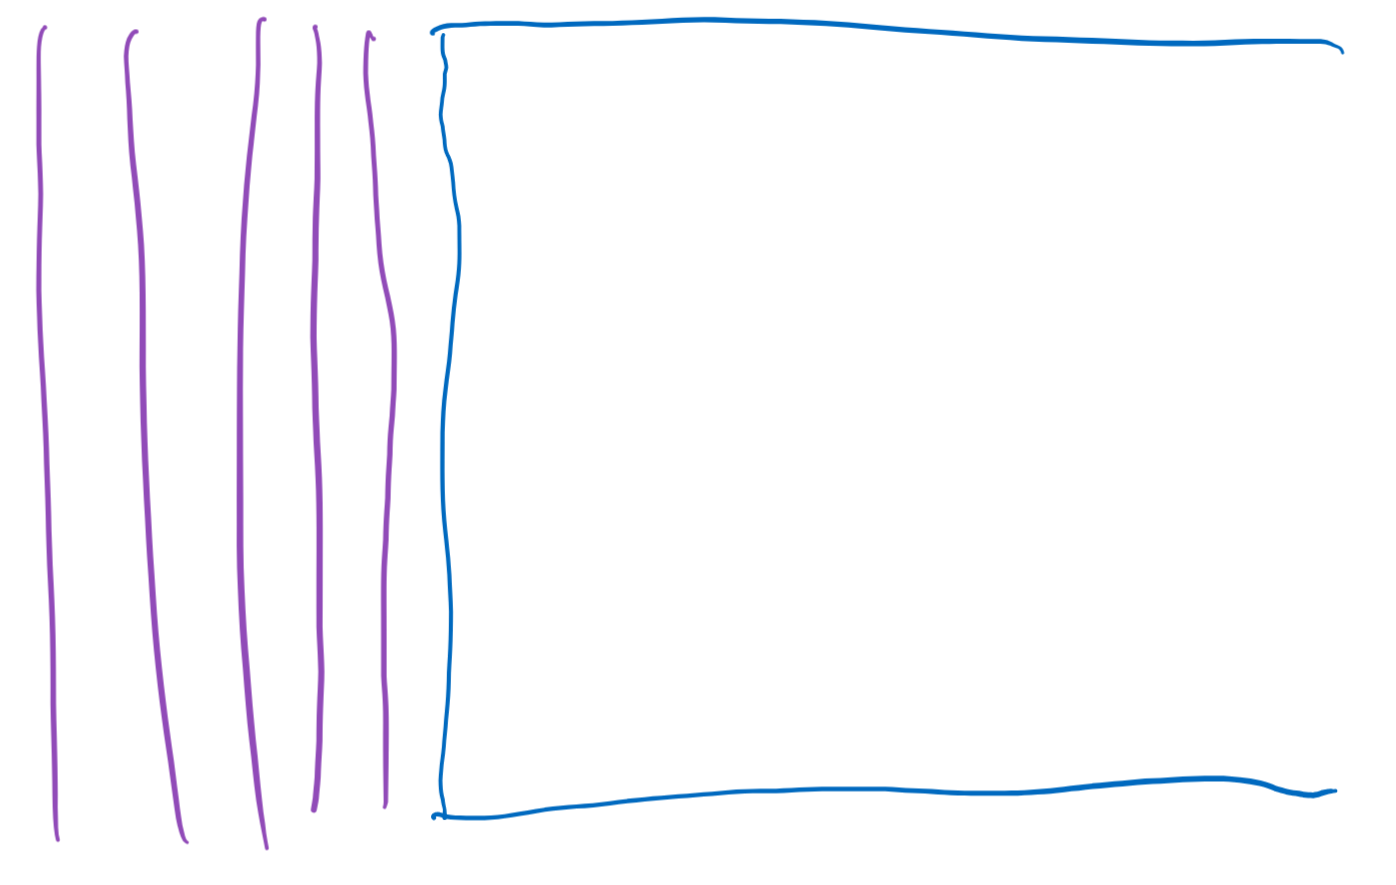
\includegraphics[width=.70\textwidth]{Foliation example.png}
	\label{fig:Foliation example}
\end{figure}


\end{frame}

%{
%\setbeamertemplate{footline}
%{
  %\leavevmode%
  %\hbox{%
  %\begin{beamercolorbox}[wd=.09\paperwidth,ht=2.25ex,dp=1ex,center]{author in head/foot}%
    %\usebeamerfont{author in head/foot}
		%Sources
  %\end{beamercolorbox}%
  %\begin{beamercolorbox}[wd=.91\paperwidth,ht=2.25ex,dp=1ex,center]{title in head/foot}%
    %\usebeamerfont{title in head/foot}
		%Private communication with Camille Laurent-Gengoux.
  %\end{beamercolorbox}%
  %%\begin{beamercolorbox}[wd=.175\paperwidth,ht=2.25ex,dp=1ex,right]{date in head/foot}%
    %%\usebeamerfont{date in head/foot}\insertshortdate{}\hspace*{2em}
    %%%\insertframenumber{} 
		%%%/ \inserttotalframenumber\hspace*{2ex} 
  %%\end{beamercolorbox}
	%}%
  %\vskip0pt%
%}
%\begin{frame}{Why finitely generated?}
%
%\begin{figure}[htbp]
	%\centering
		%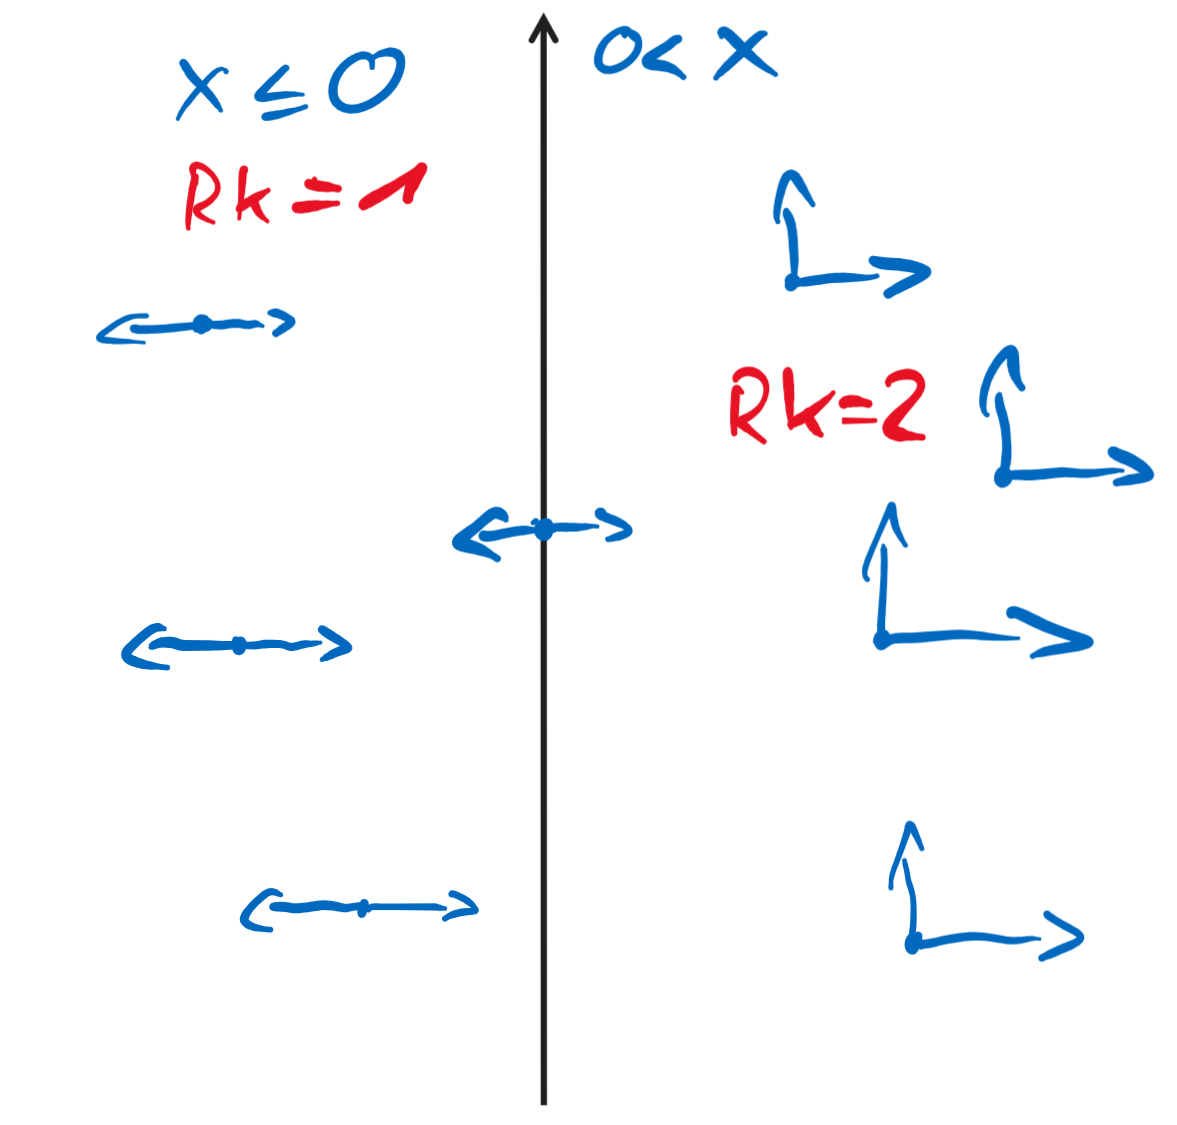
\includegraphics[width=0.50\textwidth]{Infinite comb.png}
	%\caption{Infinite Comb}
	%\label{fig:Infinite comb}
%\end{figure}
%\end{frame}
%}

\subsection{Idea: Relation to gauge theory}

\renewcommand\insertreferences{{\tiny Camille Laurent-Gengoux and Leonid Ryvkin, The holonomy of a singular leaf, \newline \textit{Selecta Mathematica 28}, no.\ 2, 45, 2022.}}

\begin{frame}
\begin{figure}[htbp]
	\centering
		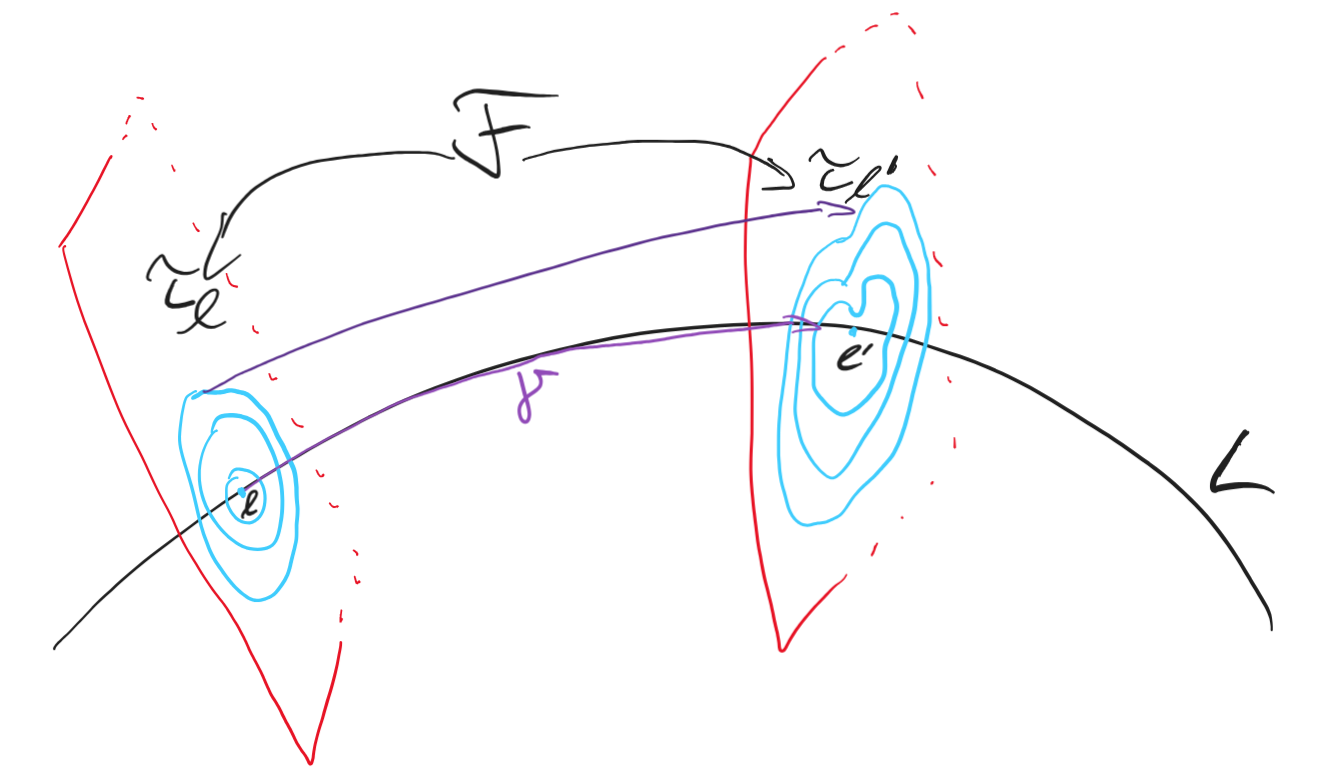
\includegraphics[width=1.00\textwidth]{Foliation connection.png}
	%\caption{$\mathcal{F}$-connections}
	\label{fig:Foliation connection}
\end{figure}

\end{frame}

\begin{frame}
\begin{figure}[htbp]
	\centering
		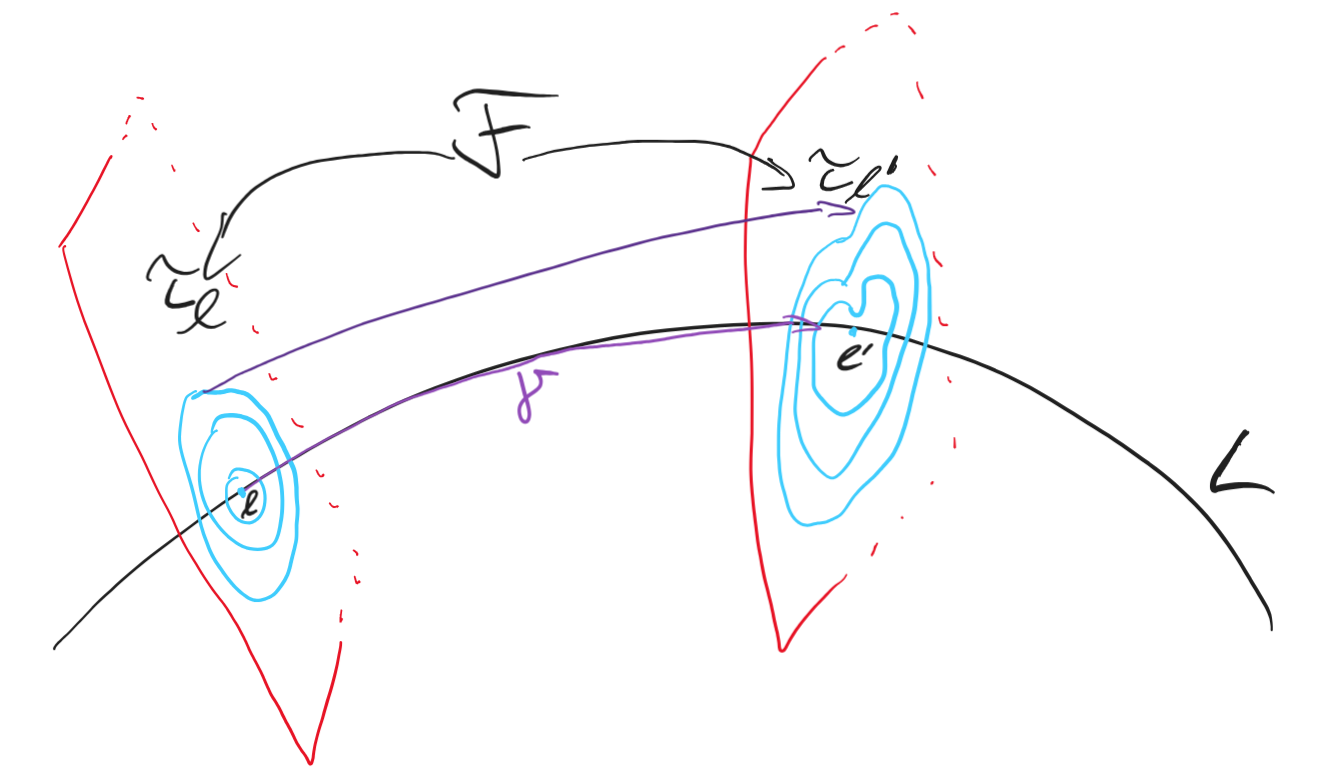
\includegraphics[width=0.50\textwidth]{Foliation connection.png}
	%\caption{$\mathcal{F}$-connections}
	\label{fig:Foliation connection Zwei}
\end{figure}

\begin{theorem}[$\mathcal{F}$-connections]
There is a connection on the normal bundle of a leaf $L$:
\begin{itemize}
	\item Horizontal vector fields are in $\mathcal{F}$.
	\item Parallel transport $\mathup{PT}_\gamma$ has values in $\mathup{Sym}(\tau_l, \tau_{l^\prime})$.
	\item For a contractible loop $\gamma_0$ at $l$: $\mathup{PT}_{\gamma_0}$ values in $\mathup{Inner}(\tau_l)$.
\end{itemize}
\end{theorem}

\end{frame}

\begin{frame}{Example of a transverse foliation $\tau$:}
%\begin{center}
\begin{minipage}[]{0.45\textwidth}
\begin{figure}
\begin{tikzpicture}
\coordinate (O) at (0,0);
\foreach \k in {1,...,4}\pgfmathparse{12*\k} \draw[fill=blue!\pgfmathresult] (O) circle (3.6-0.8*\k) node at (0, 3) {$\mathbb{S}^n$};
\fill (O) circle[radius=2pt];
\end{tikzpicture}
\end{figure}
%\end{center}
\end{minipage}
\hfill
\begin{minipage}[]{0.45\textwidth}
\begin{remark}
\begin{itemize}
	\item $\mathup{Inner}(\tau_l)$ maps each circle to itself
	\item $\mathup{Sym}(\tau_l)$ allows to exchange circles
	\item Both preserve $\tau_l$ and fix the origin
\end{itemize}
\end{remark}
\end{minipage}
\end{frame}

{
\setbeamertemplate{footline}{}

\begin{frame}{Idea}
\begin{figure}[htbp]
	\centering
		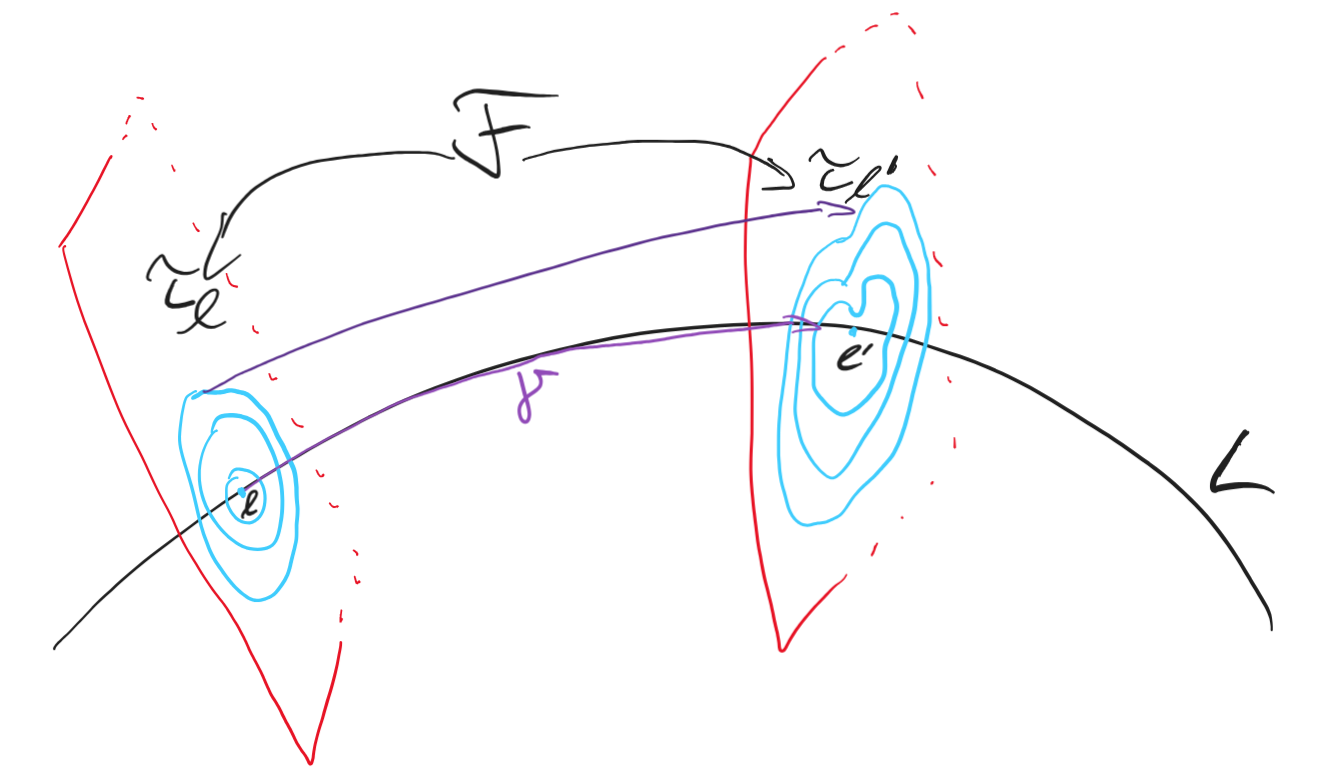
\includegraphics[width=0.5\textwidth]{Foliation connection.png}
	%\caption{$\mathcal{F}$-connections}
	\label{fig:Foliation connection Drei}
\end{figure}

\begin{idea}
Generators of $\mathcal{F}$ given by $\mathcal{F}_{\mathup{projectable}}$:
\bas
X^\uparrow + \overline{\nu},
\eas
where $X \in \mathfrak{X}(L)$, $X^\uparrow$ its projectable horizontal lift, $\nu \in \Gamma(\mathrm{inner}(\tau))$ and $\overline{\nu}$ its fundamental vector field.
\pause

\end{idea}
\end{frame}

\begin{frame}
\begin{figure}[htbp]
	\centering
		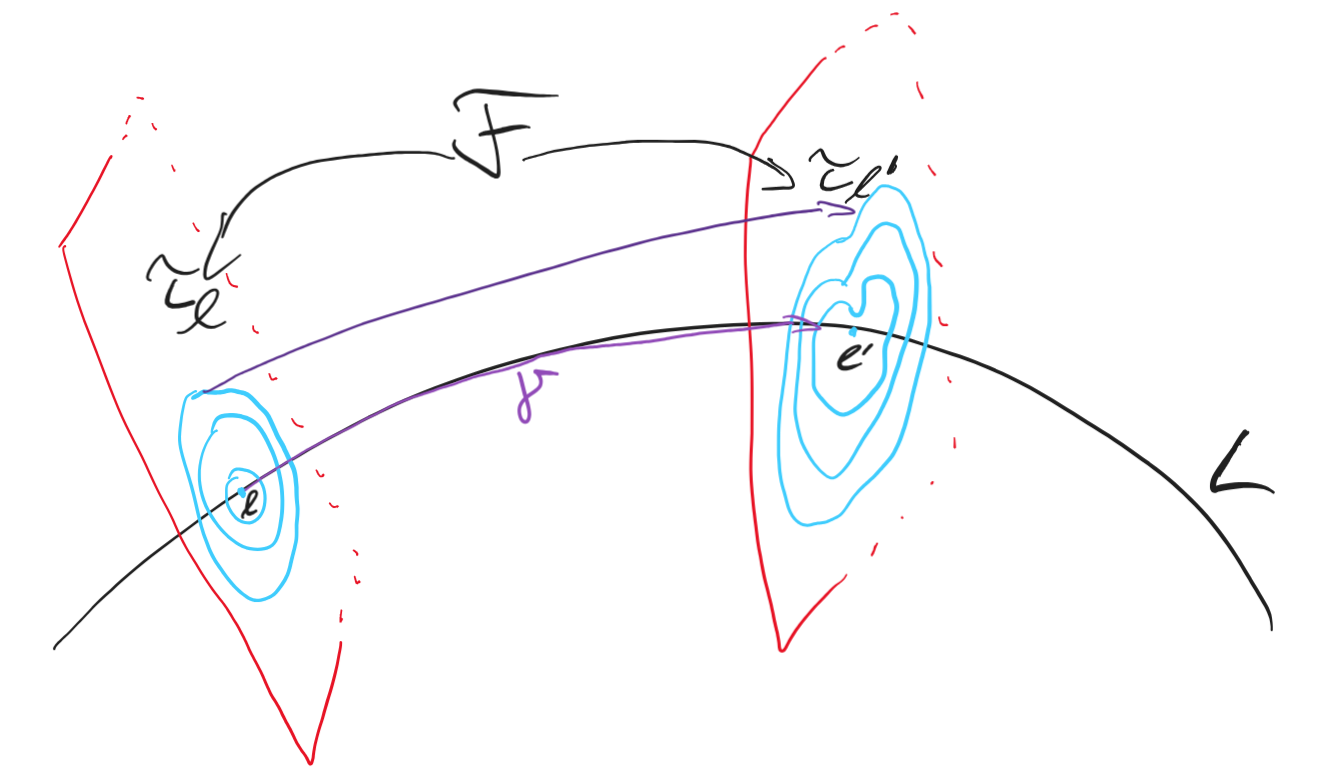
\includegraphics[width=0.5\textwidth]{Foliation connection.png}
	%\caption{$\mathcal{F}$-connections}
	\label{fig:Foliation connection Vier}
\end{figure}
\begin{idea}
Fix $l$ and given $\tau_l$: Reconstruct $\mathcal{F}$.
\bas
\mleft[ X^\uparrow + \overline{\nu}, {X^\prime}^\uparrow + \overline{\mu} \mright]
&=
\mleft[ X, X' \mright]^\uparrow + 
%\overline{\vphantom{d}
\dots
%}
\\
&=
\underbrace{\mleft[ X^\uparrow, {X^\prime}^\uparrow \mright]}_{\rightsquigarrow \text{ curvature}}
	+ \underbrace{\mleft[ X^\uparrow, \overline{\mu} \mright]
	- \mleft[ {X^\prime}^\uparrow, \overline{\nu} \mright]}_{\rightsquigarrow \text{ connection}}
	+ \overline{\mleft[ \nu, \mu \mright]}
\eas
\end{idea}
\end{frame}
}

%\section{Curved Yang-Mills gauge theory}
\subsection{Principal bundles based on Lie group bundle actions}
{
\setbeamertemplate{footline}{}

\begin{frame}
\thispagestyle{empty}
\begin{center}
\textbf{\Large Curved Yang-Mills gauge theory}
\end{center}
\end{frame}

\begin{frame}
\textbf{Curved Yang-Mills gauge theories:}
\begin{table}[h!]
	\centering
		\begin{tabular}{c c} 
			%\rowcolor{gray}
			Classical & Curved \\
			%Infinitesimal & Lie algebra $\mathfrak{g}$ & LAB\footnote{LAB = Lie algebra bundle} $\mathcal{g}$ \\
			%\rowcolor{Gray}
			Lie group $G$ & \textcolor[rgb]{1,0.41,0.13}{Lie group bundle
			%\footnote{LGB = Lie group bundle} 
			$\mathcal{G}$}
		\end{tabular}
\end{table}

\begin{center}
	\begin{tikzcd}[ampersand replacement=\&]
	G \arrow{r} \& \mathcal{G} \arrow{d} \\
	\& L
	\end{tikzcd}
\end{center}
\pause
\begin{remark}[Why a "curved theory"?]
Usually, the field strength $F$ is given by (abelian, for simplicity)
\bas
F
&\coloneqq
\mathrm{d}A
=
\mathrm{d}^{\nabla^0}A.
\eas
$\rightsquigarrow$ We will use a general connection $\nabla$ instead of $\nabla^0$, and $\nabla$ may not be flat.
\end{remark}
\end{frame}
}

\renewcommand\insertreferences{{\tiny  K. Mackenzie. General Theory of Lie Groupoids and Algebroids. \newline \textit{London Mathematical Society Lecture Note Series}, 213, 2005.}}

\begin{frame}
\begin{definition}[LGB actions]
\begin{center}
	\begin{tikzcd}[ampersand replacement=\&, column sep = small, row sep = small]
	 \& \mathcal{G} \arrow[bend right]{dl} \arrow{d}{\pi_{\mathcal{G}}} \\
	\mathcal{T} \arrow{r}{\phi} \& L
	\end{tikzcd}
\end{center}
A \textbf{right-action of $\mathcal{G}$ on $\mathcal{T}$} is a smooth map 
%\bas
$\mathcal{T} * \mathcal{G} \coloneqq \mathcal{T} \leftindex^{}_{\phi}\times_{\pi_{\mathcal{G}}} \mathcal{G} \to \mathcal{T}$,
$(t, g) \mapsto t \cdot g$,
%\eas
satisfying the following properties:
\ba\label{InvarianceOffUnderGAction}
\phi(t \cdot g) &= \phi(t),\\
(t \cdot g) \cdot h &= t \cdot (gh),\\
t \cdot e_{\phi(t)} &= p
\ea
for all $t \in \mathcal{T}$ and $g, h \in \mathcal{G}_{\phi(t)}$, where $e_{\phi(t)}$ is the neutral element of $\mathcal{G}_{\phi(t)}$.
\end{definition}
\end{frame}

\renewcommand\insertreferences{{\tiny Ieke Moerdijk, Janez Mrcun. Introduction to Foliations and Lie Groupoids. \newline \textit{Cambridge Studies in Advanced Mathematics 91, Cambridge University Press, Cambridge}, 2003}}

\begin{frame}
\begin{definition}[Principal bundle]
\begin{center}
	\begin{tikzcd}[ampersand replacement=\&]
	\mathcal{P} \arrow{d}{\pi_{\mathcal{P}}} \arrow{dr}{\phi} \& \arrow[bend right]{l} \mathcal{G} \arrow{d}{\pi_{\mathcal{G}}}
    %\arrow{l} G 
    \\
	L' \arrow{r}{\Psi} \& L
	\end{tikzcd}
\end{center}
A surjective submersion $\pi_{\mathcal{P}}\colon \mathcal{P} \to L'$, with $\mathcal{G}$-action
\bas
\begin{matrix}
	\textcolor[rgb]{1,0,0}{\xcancel{\mathcal{P} \times G}} &\to \mathcal{P} \\
	\mathcal{P} * \mathcal{G} &
\end{matrix}
\eas
simply transitive on $\pi_{\mathcal{P}}$-fibres of $\mathcal{P}$, and "suitable" atlas.
\end{definition}
\end{frame}

\subsection{Connections as parallel transport}
{
\setbeamertemplate{footline}{}
\begin{frame}{Connection on $\mathcal{P}$: Idea}
\begin{figure}
%\caption{Pushforwards via right-multiplication of tangent vectors}  
%\label{figure:fibre bundle}
\centering
\begin{tikzpicture}[scale=0.55]
\draw (0,-3.5) to[out=10,in=170] (4.25,-3.5) to[out=350,in=190] (8.5,-3.5);
\draw [->, draw=orange] (8.7,-3.5) -- (10.3,-3.5);
\draw (9.5,-4) node {\textcolor[rgb]{1,0.647,0}{$\Psi \colon L' \to L$}};
\draw (1.25,2.5) to[out=280,in=90](1.5,0) to[out=270,in=80] (1.25,-2.5);
\filldraw [fill=gray!20!white, draw=white] (3.5,2.5) to[out=280,in=90](3.75,0) to[out=270,in=80] (3.5,-2.5) -- (5,-2.5)  to[out=80,in=270](5.25,0) to[out=90,in=280] (5,2.5) -- cycle;
\draw (4.25,2.5) to[out=280,in=95](4.41,1) to[out=275,in=85] (4.41,-1) to[out=265,in=80] (4.25,-2.5); %draw with middle section for precise point placement

\draw (4,-1) node {\textcolor[rgb]{1,0,0}{$p$}};
\draw [<-, draw=blue] (5,1) to[out=275,in=85] (5,-1);
\draw (5.5,0) node {\textcolor[rgb]{0,0,1}{$\cdot g$}};
\filldraw [fill=red, draw=red] (4.41,1) circle (1pt);
\filldraw [fill=red, draw=red] (4.41,-1) circle (1pt);
\draw (5.75,2.5) to[out=280,in=90](6,0) to[out=270,in=80] (5.75,-2.5);
\draw (7.25,2.5) to[out=280,in=90](7.5,0) to[out=270,in=80] (7.25,-2.5);
\draw (2.75,2.475) to[out=280,in=90](3,0) to[out=270,in=80] (2.75,-2.475);

%\draw (4.75,2) node {$\mathcal{P}_x$};
%\draw (4.95,1.5) node {$\cong G$};
%\draw (9.5,-3.5) node {$M$};
\draw (5,2) node {$\mathcal{P}_U$};
\draw (3.5,-3.4) node {$($};
\filldraw [fill=red, draw=red] (4.25,-3.5) circle (1pt);
\draw (4.25,-3.9) node {\textcolor[rgb]{1,0,0}{$x$}};
\draw (5,-3.6) node {$)$};
\draw (4.25, -3) node {$U$};
\draw (0,0) node {$\mathcal{P}$};
\draw [->] (0,-0.4) -- (0,-3.1);
\draw (0.6,-1.75) node {$\pi_{\mathcal{P}}$};
\draw (3.5,1) node {\textcolor[rgb]{1,0,0}{$p \cdot g$}};
%%%%%%%%%%%%%%%%%%%%%%%%%%%%%%%%%%%%%%%%%%%%%%%%%%%%%%%%%%%%%%%%%%%%%%%%%%%%%%%%%%%%
\draw (10.5,-3.5) to[out=10,in=170] (14.75,-3.5) to[out=350,in=190] (19,-3.5); %hori M
\filldraw [fill=gray!20!white, draw=white] (14,2.5) to[out=280,in=90](14.25,0) to[out=270,in=80] (14,-2.5) -- (15.5,-2.5)  to[out=80,in=270](15.75,0) to[out=90,in=280] (15.5,2.5) -- cycle; %gray area
\draw (11.75,2.5) to[out=280,in=90](12,0) to[out=270,in=80] (11.75,-2.5); %vert line 1
\draw (14.75,2.5) to[out=280,in=90](15,0) to[out=270,in=80] (14.75,-2.5); %3
\draw (16.25,2.5) to[out=280,in=90](16.5,0) to[out=270,in=80] (16.25,-2.5); %4
\draw (17.75,2.5) to[out=280,in=90](18,0) to[out=270,in=80] (17.75,-2.5); %5

\draw (13.25,2.475) to[out=280,in=90](13.5,0) to[out=270,in=80] (13.25,-2.475); %2
\filldraw [fill=blue, draw=blue] (15,0) circle (1pt);
\draw (15.5,0) node {\textcolor[rgb]{0,0,1}{$g$}};

\draw (19,0) node {$\mathcal{G}$}; %These three lines are for LGB projection
\draw [->] (19,-0.4) -- (19,-3.1);
\draw (18.5,-1.75) node {$\pi_{\mathcal{G}}$};

\draw (15.5,2) node {$\mathcal{G}_U$};
\draw (14,-3.4) node {$($};
\filldraw [fill=red, draw=red] (14.75,-3.5) circle (1pt);
\draw (14.75,-4.2) node {\textcolor[rgb]{1,0,0}{$\Psi(x)$}};
\draw (15.5,-3.6) node {$)$};
\draw (14.75, -2.9) node {$\Psi(U)$};

\path[<-] (8.5,0) edge [bend left] (11,0);
\end{tikzpicture}
\end{figure}
\pause
But:
\bas
&&&r_g \colon \mathcal{P}_x \to \mathcal{P}_x\\
&\Rightarrow&&\mathrm{D}_pr_g \text{ only defined on vertical structure}
\eas
\end{frame}

\begin{frame}{Connection on $\mathcal{P}$: Idea}
\begin{figure}
%\caption{Pushforwards via right-multiplication of tangent vectors}  
%\label{figure:fibre bundle part two}
\centering
\begin{tikzpicture}[scale=0.55]
\draw (0,-3.5) to[out=10,in=170] (4.25,-3.5) to[out=350,in=190] (8.5,-3.5);
\draw [->, draw=orange] (8.7,-3.5) -- (10.3,-3.5);
\draw (9.5,-4) node {\textcolor[rgb]{1,0.647,0}{$\Psi \colon L' \to L$}};
\draw (1.25,2.5) to[out=280,in=90](1.5,0) to[out=270,in=80] (1.25,-2.5);
\filldraw [fill=gray!20!white, draw=white] (3.5,2.5) to[out=280,in=90](3.75,0) to[out=270,in=80] (3.5,-2.5) -- (5,-2.5)  to[out=80,in=270](5.25,0) to[out=90,in=280] (5,2.5) -- cycle;
\draw (4.25,2.5) to[out=280,in=95](4.41,1) to[out=275,in=85] (4.41,-1) to[out=265,in=80] (4.25,-2.5); %draw with middle section for precise point placement

\draw (4,-1) node {\textcolor[rgb]{1,0,0}{$p$}};
\draw [<-, draw=blue] (5,1) to[out=275,in=85] (5,-1);
\draw [<-, draw=blue] (4.8,1) to[out=275,in=85] (4.8,-1);
\draw [<-, draw=blue] (4.6,1) to[out=275,in=85] (4.6,-1);
\draw (5.5,0) node {\textcolor[rgb]{0,0,1}{$\cdot \sigma$}};
\filldraw [fill=red, draw=red] (4.41,1) circle (1pt);
\filldraw [fill=red, draw=red] (4.41,-1) circle (1pt);
\draw (5.75,2.5) to[out=280,in=90](6,0) to[out=270,in=80] (5.75,-2.5);
\draw (7.25,2.5) to[out=280,in=90](7.5,0) to[out=270,in=80] (7.25,-2.5);
\draw (2.75,2.475) to[out=280,in=90](3,0) to[out=270,in=80] (2.75,-2.475);

%\draw (4.75,2) node {$\mathcal{P}_x$};
%\draw (4.95,1.5) node {$\cong G$};
%\draw (9.5,-3.5) node {$M$};
\draw (5,2) node {$\mathcal{P}_U$};
\draw (3.5,-3.4) node {$($};
\filldraw [fill=red, draw=red] (4.25,-3.5) circle (1pt);
\draw (4.25,-3.9) node {\textcolor[rgb]{1,0,0}{$x$}};
\draw (5,-3.6) node {$)$};
\draw (4.25, -3) node {$U$};
\draw (0,0) node {$\mathcal{P}$};
\draw [->] (0,-0.4) -- (0,-3.1);
\draw (0.6,-1.75) node {$\pi_{\mathcal{P}}$};
\draw (3.5,1) node {\textcolor[rgb]{1,0,0}{$r_\sigma(p)$}};
%%%%%%%%%%%%%%%%%%%%%%%%%%%%%%%%%%%%%%%%%%%%%%%%%%%%%%%%%%%%%%%%%%%%%%%%%%%%%%%%
\draw (10.5,-3.5) to[out=10,in=170] (14.75,-3.5) to[out=350,in=190] (19,-3.5); %hori M
\filldraw [fill=gray!20!white, draw=white] (14,2.5) to[out=280,in=90](14.25,0) to[out=270,in=80] (14,-2.5) -- (15.5,-2.5)  to[out=80,in=270](15.75,0) to[out=90,in=280] (15.5,2.5) -- cycle; %gray area
\draw (11.75,2.5) to[out=280,in=90](12,0) to[out=270,in=80] (11.75,-2.5); %vert line 1
\draw (14.75,2.5) to[out=280,in=90](15,0) to[out=270,in=80] (14.75,-2.5); %3
\draw (16.25,2.5) to[out=280,in=90](16.5,0) to[out=270,in=80] (16.25,-2.5); %4
\draw (17.75,2.5) to[out=280,in=90](18,0) to[out=270,in=80] (17.75,-2.5); %5

\draw (13.25,2.475) to[out=280,in=90](13.5,0) to[out=270,in=80] (13.25,-2.475); %2
\draw [draw=blue] (14.25,0) to[out=10,in=170] (15,0) to[out=350,in=190] (15.75,0);
%\filldraw [fill=blue, draw=blue] (15,0) circle (1pt);
\draw (13.9,0) node {\textcolor[rgb]{0,0,1}{$\sigma$}};

\draw (19,0) node {$\mathcal{G}$}; %These three lines are for LGB projection
\draw [->] (19,-0.4) -- (19,-3.1);
\draw (18.5,-1.75) node {$\pi_{\mathcal{G}}$};

\draw (15.5,2) node {$\mathcal{G}_U$};
\draw (14,-3.4) node {$($};
\filldraw [fill=red, draw=red] (14.75,-3.5) circle (1pt);
\draw (14.75,-4.2) node {\textcolor[rgb]{1,0,0}{$\Psi(x)$}};
\draw (15.5,-3.6) node {$)$};
\draw (14.75, -2.9) node {$\Psi(U)$};

\path[<-] (8.5,0) edge [bend left] (11,0);
\end{tikzpicture}
\end{figure}

\bas
\text{Use } \sigma \in \Gamma(\mathcal{G})\colon r_\sigma(p) \coloneqq p \cdot \sigma_{\Psi(x)}
\eas
\end{frame}

\begin{frame}{Connection on $\mathcal{P}$: Revisiting the classical setup}
\setbeamercovered{invisible}
	\begin{minipage}[]{0.45\textwidth} 
	If $\mathcal{P}$ a typical principal bundle ($\mathcal{G}$ trivial, $\sigma \equiv g$ constant), and \textcolor[rgb]{0,0.58,0}{$H$} a connection:
	\begin{figure}
	\begin{tikzpicture}[scale=1.2]
		%Gray area
		\filldraw [fill=gray!20!white, draw=white] (3.5,2.5) to[out=280,in=95](3.66,1) to[out=275,in=85] (3.66,-1) to[out=265,in=80] (3.5,-2.5) -- (5,-2.5) to[out=80, in=265] (5.16, -1) to[out=85, in=275] (5.16, 1) to[out=95,in=280] (5,2.5) -- cycle;
		%lines
		\draw (4.25,2.5) to[out=280,in=95](4.41,1) to[out=275,in=85] (4.41,-1) to[out=265,in=80] (4.25,-2.5);
		\definecolor{darkgreen}{rgb}{0,0.58,0}
		\draw [draw=darkgreen] (3.66,-1) to[out=280,in=200] (4.41,-1) to[out=20,in=100] (5.16, -1);
		\draw [draw=darkgreen] (3.66,1) to[out=280,in=200] (4.41,1) to[out=20,in=100] (5.16,1);
		%Auxiliary stuff like arrows and dots
		\filldraw [fill=red, draw=red] (4.41,1) circle (1pt);
		\filldraw [fill=red, draw=red] (4.41,-1) circle (1pt);
		\draw [<-, draw=blue] (5.16,1) to[out=275,in=85] (5.16,-1);
		\draw [->, thick] (4.41,-1) -- (4.71,-0.88);
		%\draw [->] (4.41,1) -- (4.63,2);
		\draw [->, thick] (4.41,1) -- (4.71,1.12);
		%\draw [<-,dotted,thick] (4.63,2) -- (4.71,1.12);
		%Labels
		\draw (3.2,1) node {\textcolor[rgb]{0,0.58,0}{$H_{p \cdot g}$}};
		\draw (3.2,-1) node {\textcolor[rgb]{0,0.58,0}{$H_p$}};
		\draw (5.5,0) node {\textcolor[rgb]{0,0,1}{$\cdot g$}};
		\draw (3,2.2) node {$\mathcal{P}_U$};
		\draw (4.71,-0.6) node {$X$};
		\draw (5,1.4) node {$\mathrm{D}_pr_g(X)$};
		%\draw (5.5,1.56) node {$\thicksim \mathrm{D}_x\sigma(X)$};
		%Text
	\end{tikzpicture}
	\end{figure}
	\end{minipage}\hfill
	\pause
	\begin{minipage}[]{0.45\textwidth} 
	\begin{remark}[Integrated case]
	Parallel transport $\mathup{PT}^{\mathcal{P}}_\gamma$ in $\mathcal{P}$:
		\bas
		%\mathrm{D}_p r_g (X)
		%&=
		%\mleft.\frac{\mathrm{d}}{\mathrm{d}t}\mright|_{t=0}\mleft( \alpha \cdot g \mright),
		\mathup{PT}^{\mathcal{P}}_\gamma(p \cdot g)
		&=
		\mathup{PT}^{\mathcal{P}}_\gamma(p) \cdot g
		%\\
		%&=
		%\mathup{PT}^{\mathcal{P}}_\alpha(p) \cdot \mathup{PT}^{\mathcal{G}}_\alpha (g)
		\eas
		where $\gamma:I \to L'$ is a base path 
	\end{remark}
	\end{minipage}
\end{frame}
%
%{
%\setbeamertemplate{footline}{}

\begin{frame}{Connection on $\mathcal{P}$: General case}
	\begin{remark}[Integrated case]
	Ansatz: Introduce connection on $\mathcal{G}$,
		\bas
		\mathup{PT}^{\mathcal{P}}_\gamma(p \cdot g)
		&=
		\mathup{PT}^{\mathcal{P}}_\gamma(p) \cdot \mathup{PT}^{\mathcal{G}}_{\Psi \circ \gamma} (g).
		\eas
	\end{remark}
	\pause
\begin{BackToTheRoots}
\begin{enumerate}
	\item $\mathcal{G} \cong L \times G$
	\item Equip $\mathcal{G}$ with canonical flat connection
\end{enumerate}
\end{BackToTheRoots}
\end{frame}
\subsection{General notion of Ehresmann and Yang-Mills connections}
\begin{frame}
\begin{definition}[Ehresmann/Yang-Mills connection, {[C.\ L.-G., S.-R.\ F.]}]
A surjective submersion $\pi_{\mathcal{T}} \colon \mathcal{T} \to L'$ so that one has a commuting diagram
\begin{center}
	\begin{tikzcd}[ampersand replacement=\&]
	\mathcal{T} \arrow[swap]{d}{\pi_{\mathcal{T}}} \arrow{dr}{\phi} \& \arrow[bend right]{l} \mathcal{G} \arrow{d}{\pi_{\mathcal{G}}}
    %\arrow{l} G 
    \\
	L' \arrow{r}{\Psi} \& L
	\end{tikzcd}
\end{center}
\begin{enumerate}
	\item \textbf{Ehresmann connection:} $\mathcal{G}$ preserving $\pi_{\mathcal{T}}$ and
	\bas
	\mathup{PT}_\gamma^{\mathcal{T}}(t \cdot g)
	&=
	\mathup{PT}_\gamma^{\mathcal{T}}(t)
	\cdot
	\mathup{PT}_{\Psi\circ\gamma}^{\mathcal{G}}(g)
	\eas
	\item \textbf{Yang-Mills connection:} Additionally
	\bas
	\mathup{PT}_{\gamma_0}^{\mathcal{T}}(t)
	&=
	t \cdot g_{\gamma_0}
	\eas
	for some $g_{\gamma_0} \in \mathcal{G}_{\phi(t)}$, where $\gamma_0$ is a contractible loop.
\end{enumerate}
\end{definition}
\end{frame}

\begin{frame}
\begin{definition}[Multiplicative YM connection, {[S.-R.\ F.]}]
On $\mathcal{G}$ there is also the notion of \textbf{multiplicative Yang-Mills connections}, that is,
\bas
\mathup{PT}_\gamma^{\mathcal{G}}(q \cdot g)
&=
\mathup{PT}_\gamma^{\mathcal{G}}(q)
\cdot
\mathup{PT}_{\gamma}^{\mathcal{G}}(g),
\\
\mathup{PT}_{\gamma_0}^{\mathcal{G}}(q)
&=
g_{\gamma_0} \cdot q \cdot g_{\gamma_0}^{-1}
\eas
\end{definition}

\pause

\begin{definition}[Principal bundle connection, {[S.-R.\ F.]}]
\begin{itemize}
	\item On $\mathcal{G}$: Multiplicative Yang-Mills connection
	\item On $\mathcal{P}$: Ehresmann connection
\end{itemize}
\end{definition}

\pause

\begin{remark}[{[S.-R.\ F.]}]
This gives rise to a generalised gauge theory by contracting the involved curvatures.
\end{remark}
\end{frame}
}
%
%\subsection{Connection and curvature}
%
%{
%\setbeamertemplate{footline}{}

\renewcommand\insertreferences{{\tiny For differential: Marius Crainic, Maria Amelia Salazar, and Ivan Struchiner. Multiplicative forms and Spencer operators. \newline \textit{Mathematische Zeitschrift}, 279(3):939–979, 2015.}}

\begin{frame}
\begin{remark}
There is a simplicial differential $\delta$ on $\mathcal{G} \stackrel{\pi_{\mathcal{G}}}{\to} L$ with Lie algebra bundle $\mathcal{g}$
\bas
\delta: \Omega^\bullet( \underbrace{\mathcal{G} * \dotsc * \mathcal{G}}_{k \text{ times}}; \pi_{\mathcal{G}}^*\mathcal{g} )
&\to
\Omega^\bullet( \underbrace{\mathcal{G} * \dotsc * \mathcal{G}}_{k + 1 \text{ times}}; \pi_{\mathcal{G}}^*\mathcal{g} )
\eas
such that the definition of the multiplicative Yang-Mills connection is equivalent to the \textbf{compatibility conditions}
\begin{itemize}
	\item Connection closed
	\item Curvature exact ([S.-R.\ F.])
\end{itemize}
\end{remark}
\end{frame}

\renewcommand\insertreferences{{\tiny For the first equation: Camille Laurent-Gengoux, Mathieu Stiénon, and Ping Xu. Non-abelian differentiable gerbes. \newline \textit{Advances in Mathematics}, 220(5):1357–1427, 2009.}}

\begin{frame}
\begin{remark}
On the Lie algebra bundle $\mathcal{g}$ we have a connection $\nabla^{\mathcal{G}}$ with 
\bas
\nabla^{\mathcal{G}}\mleft( \mleft[ \mu, \nu \mright]_{\mathcal{g}} \mright)
&=
\mleft[ \nabla^{\mathcal{G}} \mu, \nu \mright]_{\mathcal{g}}
	+ \mleft[ \mu, \nabla^{\mathcal{G}} \nu \mright]_{\mathcal{g}},
\\
R_{\nabla^{\mathcal{G}}}
&=
\mathrm{ad} \circ \zeta. \qquad \text{ ([S.-R.\ F.])}
\eas
\end{remark}
\pause
\begin{example}
Given a short exact sequence of algebroids 
\begin{center}
	\begin{tikzcd}[ampersand replacement=\&]
	\mathcal{g} \arrow[hook]{r}
	\& E \arrow[two heads]{r}
	\& \mathrm{T}L
	\end{tikzcd}
\end{center}
with splitting $\chi \colon \mathrm{T}L \to E$, then
\bas
\nabla^{\mathcal{G}}_X \nu
&=
\mleft[ \chi(X), \nu \mright]_E,
\\
\zeta\mleft( X, X' \mright)
&=
\mleft[ \chi(X), \chi(X') \mright]_E
	- \chi\mleft( [X, X'] \mright).
\eas
\end{example}
\end{frame}





%\section{Foliations and Yang-Mills connections}
\subsection{Reconstructing Foliations}
{
\setbeamertemplate{footline}{}

\begin{frame}
\thispagestyle{empty}
\begin{center}
\textbf{\Large Going back to foliations}
\end{center}
\end{frame}

\begin{frame}
\begin{theorem}[{[C.\ L.-G., S.-R.\ F.]}]
Given a multiplicative Yang-Mills connection on $\mathcal{G}$ and a Yang-Mills connection on $\mathcal{T}$, then there is a natural foliation on $\mathcal{T}$ generated by 
\bas
X^\uparrow + \overline{\nu},
\eas
where $X \in \mathfrak{X}(L)$ and $\nu \in \Gamma(\mathcal{g})$.
\end{theorem}
\pause
\begin{proof}
We have
\bas
\mleft[ X^\uparrow, \overline{\nu} \mright]
&=
\overline{ \nabla^{\mathcal{G}}_X \nu },
\\
\mleft[ X^\uparrow, {X^\prime}^\uparrow \mright]
&=
\mleft[ X, X^\prime \mright]^\uparrow
	+ \overline{\zeta\mleft(X, X^\prime\mright)},
\eas
where $\zeta \in \Omega^2(L; \mathcal{g})$.	
\end{proof}
\end{frame}

\begin{frame}
\begin{idea}[Leaf $L$ simply connected]
Fix a point $l \in L$ with transverse model $\mleft(\mathbb{R}^d, \tau_l\mright)$:
\begin{enumerate}
	\item $G = \mathrm{Inn}(\tau_l)$
	\pause
	\item $P$ a principal $G$-bundle, equipped with an ordinary connection
	%\pause
	%\item 
	\pause
	\item $\mathcal{G} \coloneqq (P \times G) \Big/ G$, the \textbf{inner group bundle}
	\pause
	\item $\mathcal{T} \coloneqq \mleft(P \times \mathbb{R}^d\mright) \Big/ G$, the \textbf{normal bundle}
\end{enumerate}
\end{idea}

\pause

\begin{remark}
\begin{itemize}
	\item Think of the induced connection on $\mathcal{T}$ as the $\mathcal{F}$-connection.
	\item $\mathcal{G}$ acts on $\mathcal{T}$ (canonically from the left).
\end{itemize}
\end{remark}

\end{frame}

\begin{frame}
\begin{proposition}[{[C.\ L.-G., S.-R.\ F.]}]
The associated connection on $\mathcal{G}$ is a multiplicative Yang-Mills connection and the one on $\mathcal{T}$ is a corresponding Yang-Mills connection.
\end{proposition}

\begin{remark}
Thus, we have a singular foliation on $\mathcal{T}$, which, by construction, admits $L$ as a leaf and $\tau_l$ as transverse data.
\end{remark}
\end{frame}

{
\setbeamertemplate{footline}{}

\subsection{Independency of choice of connection}

\begin{frame}
\begin{lemma}[{[C.\ L.-G., S.-R.\ F.]}]
$\mathcal{P} \coloneqq (P \times P) \Big/ G$, the \textbf{Atiyah groupoid}, is a principal $\mathcal{G}$-bundle
\begin{center}
	\begin{tikzcd}[ampersand replacement=\&]
	\mathcal{P} \arrow{dr}{s} \arrow[swap]{d}{(t, s)} 
	\& \arrow[bend right]{l} \mathcal{G} \arrow{d}
    \\
	L \times L \arrow[swap]{r}{\mathrm{pr}_2} \& L
	\end{tikzcd}
\end{center}
where $t$ and $s$ are the target and source arrows, respectively.

A connection on $P$ induces an Ehresmann connection on $\mathcal{P}$.
\end{lemma}
\end{frame}

\begin{frame}
\begin{definition}[Associated bundles, {[C.\ L.-G., S.-R.\ F.]}]
\begin{center}
	\begin{tikzcd}[ampersand replacement=\&]
	\mathcal{P} \arrow[swap]{d}{(t, s)} \arrow{dr}{s} 
	\& \arrow[bend right]{l} \mathcal{G} \arrow{d}{\pi_{\mathcal{G}}} \arrow[bend left]{dr}
    \\
	L' \arrow{r}{\mathup{pr}_2} \& L \& \arrow{l}{\pi_{\mathcal{T}}} \mathcal{T}
	\end{tikzcd}
\end{center}
Equivalence relation on $\mathcal{P} \leftindex^{}_{s} \times_{\pi_{\mathcal{T}}} \mathcal{T}$
\bas
(p, t) &\sim \mleft( p \cdot g, g^{-1} \cdot t \mright)
\eas
defines the \textbf{associated bundle $\mathcal{P} \tilde{\times} \mathcal{T}$} over $L'$.
\end{definition}
\end{frame}

\begin{frame}
\begin{theorem}[Associated connection, {[C.\ L.-G., S.-R.\ F.]}]
\bas
\mathup{PT}^{\mathcal{P} \tilde{\times} \mathcal{T}}_\gamma [p, t]
&\coloneqq
\mleft[ \mathup{PT}^{\mathcal{P}}_\gamma(p), \mathup{PT}^{\mathcal{T}}_{\mathrm{pr}_2 \circ \gamma} (t) \mright]
\eas
is a well-defined connection. 
\end{theorem}
%\begin{remark}
%In the case of Yang-Mills: It is reasonable to assume that the connection on $\mathcal{G}$ is then also Yang-Mills.
%\end{remark}
\pause
\begin{remark}[{[C.\ L.-G., S.-R.\ F.]}]
Associated connection independent of the choice of connection on $P$!
\end{remark}
\end{frame}
}

%\begin{frame}
%$\mathcal{P}$ comes with two natural projections to $L$, denoted by $t$ and $s$
%\begin{center}
	%\begin{tikzcd}[ampersand replacement=\&]
	%\mathcal{P} \arrow{dr}{s} \arrow[swap]{d}{(t, s)} 
	%\& \arrow[bend right]{l} \mathcal{G} \arrow{d} \arrow[bend left]{dr}
    %\\
	%L \times L \arrow[swap]{r}{\mathrm{pr}_2} \& L \& \arrow{l}{\pi_{\mathcal{T}}} \mathcal{T}
	%\end{tikzcd}
%\end{center}
%\pause
%This extends to the associated bundle
%\begin{center}
	%\begin{tikzcd}[ampersand replacement=\&]
	%\mathcal{P} \tilde{\times} \mathcal{T} \arrow[swap]{d}{(t, s)} \arrow{dr}{s} \arrow{r}
	%\& \arrow{d}{\pi_{\mathcal{T}}} \mathcal{T}
  %\\
	%L \times L \arrow[swap]{r}{\mathrm{pr}_2} \& L 
	%\end{tikzcd}
%\end{center}
%
%\pause
%
%
%\end{frame}

\begin{frame}
%\begin{definition}[Bisections]
%\begin{center}
	%\begin{tikzcd}[ampersand replacement=\&]
    %\mathcal{P} \leftindex^{}_{s}\times_{\pi_{\mathcal{T}}} \mathcal{T} \arrow{r}
    %\arrow[shift left=1ex]{d}{s} \arrow[shift right=1ex, swap]{d}{t}
    %\& \mathcal{P} \tilde{\times} \mathcal{T}
    %\arrow[shift left=1ex]{d}{s} \arrow[shift right=1ex, swap]{d}{t}
    %\\
    %L \arrow[equal]{r} \& L
   %\end{tikzcd}
%\end{center}
%We call a \textbf{bisection} a section $\sigma$ of $t$ so that $s \circ \sigma$ is a diffeomorphism of $L$. This carries a structure as a group.
%\end{definition}
Explicitly, one possible way:

\begin{remark}
Corresponding to $\mathcal{P}$ there is an Atiyah sequence:
\begin{center}
\begin{tikzcd}[ampersand replacement=\&]
	\mathup{Ad}(P)
	\arrow[hook]{r}
	\&
	\mathup{At}(P)
	\arrow[two heads]{r}
	\&
	\mathup{T}L
	\end{tikzcd}
\end{center}
Via pullback to $\mathcal{T}$ we have a transitive algebroid over $\mathcal{T}$:
\begin{center}
\begin{tikzcd}[ampersand replacement=\&]
	\pi_{\mathcal{T}}^!\mathup{Ad}(P)
	\arrow[hook]{r}
	\&
	\pi_{\mathcal{T}}^!\mathup{At}(P)
	\arrow[two heads]{r}
	\&
	\mathup{T}\mathcal{T}
	\end{tikzcd}
\end{center}
\end{remark}

\pause

\begin{remark}
Observe
\bas
\pi_{\mathcal{T}}^!\mathup{At}(P) \subset 
\mathrm{T} \mleft( \mathcal{P} \leftindex^{}_{s}\times_{\pi_{\mathcal{T}}} \mathcal{T} \mright)
\eas
\end{remark}
\end{frame}

\begin{frame}
$\mathup{Ad}(P)$ and $\mathup{At}(P)$ the adjoint and Atiyah bundle of $P$, respectively:
%$\mathbb{H}$ the horizontal distribution on $\mathcal{P} \tilde{\times} \mathcal{T}$:
\begin{center}
	\begin{tikzcd}[ampersand replacement=\&]
	\Gamma_{\mathup{parallel}}^{\mathup{symmetric}}\mleft( \pi_{\mathcal{T}}^!\mathup{Ad}(P) \mright)
	\arrow[hook]{r} \arrow{d}
	\&
	\Gamma_{\mathup{parallel}}^{\mathup{symmetric}}\mleft( \pi_{\mathcal{T}}^!\mathup{At}(P) \mright)
	\arrow[two heads]{r} \arrow{d}
	\&
	\mathfrak{X}(L) \arrow[equal]{d}
	\\
	\tau
	\arrow[hook]{r}
	\&
	\mathcal{F}_{\mathup{projectable}}
	\arrow[two heads]{r}
	\&
	\mathfrak{X}(L)
	\end{tikzcd}
\end{center}

%\begin{remark}
%Why Yang-Mills connections?
%\bas
%\text{Involutive} &\leftrightarrow \text{Connection on } \mathcal{T} \text{ and } \mathcal{G} \text{ Yang-Mills}
%\eas
%\end{remark}
\end{frame}

}

\section{Future Prospects}
{
\setbeamertemplate{footline}{}
\begin{frame}
%\begin{table}[h!]
		%\begin{tabularx}{\textwidth}{X| c c} 
			%\rowcolor{gray}
			%Gauge theory & Structure \\ \hline
			%Yang-Mills & Lie group $G$ \\
			%\rowcolor{Gray}
			%Curved Yang-Mills & Lie group bundle $\mathcal{G}$ \\ 
			%Curved Yang-Mills-Higgs & Lie groupoid $\mathfrak{G}$?
		%\end{tabularx}
%\end{table}

%\begin{remark}
%$\mathup{D}t$ is related to the Atiyah algebroid of $P$, $\mathup{T}P \Big/ G$.
%\end{remark}

\begin{center}
	\begin{tikzcd}[ampersand replacement=\&]
		\& \arrow{dl} \mathcal{F} \arrow{dr} \&
		\\
		\mathup{At}(P) \& \& \text{Associated connection}
	\end{tikzcd}
\end{center}

\begin{remark}[Why \textbf{curved} gauge theory?]
\begin{itemize}
	\item Associated connection invariant under choice of $\mathcal{F}$-connection $\nabla^{\mathcal{F}}$
	\item Associated connection has the form
	\bas
	\nabla^{\mathcal{F}} + A \cdot 
	\eas
	where $A$ is the connection 1-form on $\mathcal{P}$
\end{itemize}
\end{remark}

\end{frame}
}
\thispagestyle{empty}
\topmargin -3.46 cm
\vspace*{\fill}
\begin{center}
\huge \textbf{Thank you!}
\end{center}
\vspace*{\fill}

\end{document}

